\documentclass[12pt, twoside]{book}\usepackage[]{graphicx}\usepackage[]{color}
%% maxwidth is the original width if it is less than linewidth
%% otherwise use linewidth (to make sure the graphics do not exceed the margin)
\makeatletter
\def\maxwidth{ %
  \ifdim\Gin@nat@width>\linewidth
    \linewidth
  \else
    \Gin@nat@width
  \fi
}
\makeatother

\definecolor{fgcolor}{rgb}{0.345, 0.345, 0.345}
\newcommand{\hlnum}[1]{\textcolor[rgb]{0.686,0.059,0.569}{#1}}%
\newcommand{\hlstr}[1]{\textcolor[rgb]{0.192,0.494,0.8}{#1}}%
\newcommand{\hlcom}[1]{\textcolor[rgb]{0.678,0.584,0.686}{\textit{#1}}}%
\newcommand{\hlopt}[1]{\textcolor[rgb]{0,0,0}{#1}}%
\newcommand{\hlstd}[1]{\textcolor[rgb]{0.345,0.345,0.345}{#1}}%
\newcommand{\hlkwa}[1]{\textcolor[rgb]{0.161,0.373,0.58}{\textbf{#1}}}%
\newcommand{\hlkwb}[1]{\textcolor[rgb]{0.69,0.353,0.396}{#1}}%
\newcommand{\hlkwc}[1]{\textcolor[rgb]{0.333,0.667,0.333}{#1}}%
\newcommand{\hlkwd}[1]{\textcolor[rgb]{0.737,0.353,0.396}{\textbf{#1}}}%
\let\hlipl\hlkwb

\usepackage{framed}
\makeatletter
\newenvironment{kframe}{%
 \def\at@end@of@kframe{}%
 \ifinner\ifhmode%
  \def\at@end@of@kframe{\end{minipage}}%
  \begin{minipage}{\columnwidth}%
 \fi\fi%
 \def\FrameCommand##1{\hskip\@totalleftmargin \hskip-\fboxsep
 \colorbox{shadecolor}{##1}\hskip-\fboxsep
     % There is no \\@totalrightmargin, so:
     \hskip-\linewidth \hskip-\@totalleftmargin \hskip\columnwidth}%
 \MakeFramed {\advance\hsize-\width
   \@totalleftmargin\z@ \linewidth\hsize
   \@setminipage}}%
 {\par\unskip\endMakeFramed%
 \at@end@of@kframe}
\makeatother

\definecolor{shadecolor}{rgb}{.97, .97, .97}
\definecolor{messagecolor}{rgb}{0, 0, 0}
\definecolor{warningcolor}{rgb}{1, 0, 1}
\definecolor{errorcolor}{rgb}{1, 0, 0}
\newenvironment{knitrout}{}{} % an empty environment to be redefined in TeX

\usepackage{alltt}\usepackage[]{graphicx}\usepackage[]{color}

\usepackage{alltt}\usepackage[]{graphicx}\usepackage[]{color}
\usepackage[utf8]{inputenc}
\usepackage[spanish]{babel}
\usepackage{fancyhdr}
\usepackage{lastpage}
\usepackage{lscape} %Para seleccionar páginas horizontales 
\usepackage[cc]{titlepic} 
\usepackage[hidelinks]{hyperref}  %Para links ocultos
\usepackage{url} %Para direcciones web
\usepackage[makeroom]{cancel}
\pagestyle{fancy}
\usepackage{multicol} % muchas columnas
\usepackage{booktabs} % midrule, bottomrule
\usepackage{titlesec}
\titlespacing\section{0pt}{12pt plus 4pt minus 2pt}{0pt plus 2pt minus 2pt}
\titlespacing\subsection{0pt}{12pt plus 4pt minus 2pt}{0pt plus 2pt minus 2pt}
\titlespacing\subsubsection{0pt}{12pt plus 4pt minus 2pt}{0pt plus 2pt minus 2pt} 
\setcounter{tocdepth}{3}
\setcounter{secnumdepth}{3}
\usepackage{blindtext}
\usepackage{listings} % Para escribir texto plano 
\let\bold\boldsymbol
\let\bf\mathbf


\parindent=0pt % Para el uso de sangrías
\parskip=\medskipamount

\fancyhf{}
 \setcounter{page}{1}
%\rfoot{Página \thepage \hspace{1pt} de \pageref{LastPage}}
\setcounter{section}{0}

\usepackage[caption=false]{subfig}
\usepackage{blindtext}  %Texo sin sentido
\usepackage{amsmath} \newenvironment{smatrix}{\left(\begin{smallmatrix}}{\end{smallmatrix}\right)} %SMALL
\usepackage{amsthm}
\usepackage{amsfonts}
\DeclareMathOperator{\sgn}{sgn} %Para formalizar la función signo 
\usepackage{enumerate}
\usepackage{dsfont} %Para usar una indicadora
\numberwithin{equation}{section}
\usepackage{xcolor}
\usepackage[backend=bibtex]{biblatex}
\bibliography{biblio.bib}
\usepackage{booktabs,caption}
\usepackage[flushleft]{threeparttable}


\makeatletter
\newcommand{\distas}[1]{\mathbin{\overset{#1}{\kern\z@\sim}}}%
\newsavebox{\mybox}\newsavebox{\mysim}
\newcommand{\distras}[1]{%
  \savebox{\mybox}{\hbox{\kern3pt$\scriptstyle#1$\kern3pt}}%
  \savebox{\mysim}{\hbox{$\sim$}}%
  \mathbin{\overset{#1}{\kern\z@\resizebox{\wd\mybox}{\ht\mysim}{$\sim$}}}%
}
\makeatother
\usepackage{mdframed} %Para usar recuadros

    \usepackage{framed}

    \colorlet{shadecolor}{blue!15}

    \newtheorem{theorem}{Observación}
    \newenvironment{theo}
      {\begin{shaded}\begin{theorem}}
      {\end{theorem}\end{shaded}}
      \numberwithin{theorem}{section}

\colorlet{shadecolor}{red!15}

    \newtheorem{teorema}{Proposición}
    \newenvironment{teo}
      {\begin{shaded}\begin{teorema}}
      {\end{teorema}\end{shaded}}
      \numberwithin{teorema}{section}

\colorlet{shadecolor}{gray!15}
    \newtheorem{defi}{Definición}
    \newenvironment{defin}
      {\begin{shaded}\begin{defi}}
      {\end{defi}\end{shaded}}
      \numberwithin{defi}{section}
%\newtheorem{rexample}{Código R}[subsection]
\newtheorem{prop}{Proposición}
%\newtheorem{defi}{Definición}
\numberwithin{prop}{section}
\numberwithin{defi}{section}
\theoremstyle{plain}
\setlength{\textfloatsep}{10pt}
\usepackage{multicol}
\usepackage{float}

\usepackage[affil-it]{authblk}
\usepackage{setspace}
\usepackage{listings}

\usepackage{geometry}
\geometry{a4paper, left=3cm, right=3cm, top=3cm, bottom=3cm}
\newcommand*\rfrac[2]{{}^{#1}\!/_{#2}}
\title{Análisis de datos: Transmisión de precios}
\author{H\'ector Garrido Henr\'iquez\thanks{Ingeniero Comercial. Contacto: \texttt{hectorgarridohenriquez@gmail.com}} \\ 
Profesor: Sergio Contreras Espinoza}

\affil{Mag\'ister en Matem\'atica Menci\'on Estad\'istica \\ Universidad del B\'io-B\'io}
\IfFileExists{upquote.sty}{\usepackage{upquote}}{}

\allowdisplaybreaks
\IfFileExists{upquote.sty}{\usepackage{upquote}}{}
\IfFileExists{upquote.sty}{\usepackage{upquote}}{}
\IfFileExists{upquote.sty}{\usepackage{upquote}}{}
\begin{document}
%\SweaveOpts{concordance=TRUE}
\begin{titlepage}
\begin{center}

\includegraphics[scale=0.07]{./figure/logo.png}\\
\textsc{\Large Universidad del Bío-Bío \\[0.5cm] Facultad de Ciencias}\\[1cm] % University name
\textsc{\Large}\\[0.3cm] % Thesis type

\noindent\makebox[\linewidth]{\rule{\textwidth}{1pt}} 
{\huge Transmisi\'on Asim\'etrica de Precios en el sector de la palta en Chile:\\[0.3cm] Evidencia desde un modelo TVECM}\\[0.4cm] % Thesis title
\noindent\makebox[\linewidth]{\rule{\textwidth}{1pt}} 

\textsc{\Large}\\[0.5cm] % Thesis type

\begin{minipage}{0.45\textwidth}
\begin{flushleft} \large
\emph{Autor:}\\
Héctor Garrido Henríquez % Author name - remove the \href bracket to remove the link
\end{flushleft}
\end{minipage}
\begin{minipage}{0.45\textwidth}
\begin{flushleft} \large
\emph{Profesor(es) Guía(s):} \\
Dr. Sergio Contreras Espinoza \\ Dra. Monia Ben Kaabia 
\end{flushleft}
\end{minipage}\\[2cm]
 
\large \textit{Tesis para optar al grado de Magíster en Matemática con mención en Estadística}\\[0.3cm] % University requirement text
\textit{}\\[0.4cm]
\ Departamento de Estadística \\
[0.4cm]\ Departamento de Matemática
\\[1cm] % Research group name and department name
 
{\large \today}\\[2cm] % Date
%\includegraphics{Logo} % University/department logo - uncomment to place it
 
%\vfill
\end{center}

\end{titlepage}
\newpage



\tableofcontents

\listoffigures
\listoftables
\onehalfspacing
\chapter*{Agradecimientos}
\chapter*{Abstract}
\chapter{Introducción}


\chapter{Transmisión de precios}

Meyer, J., & Cramon‐Taubadel, S. (2004). Asymmetric price transmission: a survey. Journal of agricultural economics, 55(3), 581-611.


\chapter{Modelos y contrastes estadísticos utilizados en esta tesis}

En este capítulo se exponen los principales modelos y contrastes estadísticos utilizados en esta tesis. Se comienza por la descripción de la estimación de modelos de series de tiempo univariados según la metodología de Bde los contrastes de raíz unitaria univariantes que permiten realizar una exploración preliminar de los datos, para luego abordar la formulación del modelo de regresiones vectoriales autorregresivas (\textbf{VAR}), el modelo vectorial de corrección del error (\textbf{VECM}), el contraste de cointegración de Johansen, el modelo vectorial de corrección del error por umbrales (\textbf{TVECM}) y el contraste de Hansen y Seo (2002). Además, se aborda el problema de imputación de datos faltantes a través del filtro de Kalman. 

\section{Pronósticos de una serie temporal según la metodología Box-Jenkins}

EN ESTE APARTADO DEBO CITAR EL LIBRO DE BOX JENKINS Y REINSEL

\section{Contrastes de raíz unitaria/estacionariedad}
\subsection{Contraste de Dickey-Fuller Aumentado}

El contraste más utilizado en la investigación aplicada, dada su simplicidad, es el contraste propuesto por \cite{fuller1976} y \cite{dickey1981}. Para aplicar este contraste existen dos posibles modelos 

Si $y_{t}$ satisface la siguiente ecuación

\begin{equation}
y_{t} = \alpha+\rho y_{t-1}+\epsilon_{t}\qquad (t=1,...,n)
\end{equation}
Donde $\epsilon_{t}\sim \mathcal{N}(0,\sigma^{2})$. 

Si $y_{t}$ satisface la siguiente ecuación 

Como puede observarse en el cuadro \ref{tab-1}, existen 3 estadísticos, $\Phi_{1},\quad \Phi_{2}$ y $\Phi_{3}$, y sus respectivas hipótesis que pueden ser utilizados. Mientras $\Phi_{1}$
\begin{equation}
y_{t} = \alpha+\beta\left(t-1-\frac{1}{2}n\right)+\rho y_{t-1}+\epsilon_{t}\qquad (t=1,...,n)
\end{equation}
Donde $\epsilon_{t}\sim \mathcal{N}(0,\sigma^{2})$. 

\begin{table}[h]
\centering
\begin{threeparttable}
\caption{Hipótesis del contraste de Dickey-Fuller}
\begin{tabular}{@{}llrllll@{}}
\toprule
\multicolumn{2}{l}{Estadístico} & \multicolumn{2}{c}{$\mathcal{H}_{0}$} &
\multicolumn{2}{c}{$\mathcal{H}_{a}$} \\
\cmidrule(l){3-4} \cmidrule(l){5-6} \\
\multicolumn{2}{l}{$\tau$} & 
\multicolumn{2}{l}{$\rho =1 $} & 
\multicolumn{2}{l}{$\rho =0 $} \\
\multicolumn{2}{l}{$\Phi_{1}$} &
\multicolumn{2}{l}{$(\alpha,\rho)=(0,1)$} &
\multicolumn{2}{l}{$(\alpha,\rho)\neq(0,1)$} \\
\multicolumn{2}{l}{$\Phi_{2}$} &
\multicolumn{2}{l}{$(\alpha,\beta, \rho)=(0,0,1)$} &
\multicolumn{2}{l}{$(\alpha,\beta,\rho)\neq(0,0,1)$} \\
\multicolumn{2}{l}{$\Phi_{3}$} &
\multicolumn{2}{l}{$(\alpha,\beta, \rho)=(\alpha,0,1)$} &
\multicolumn{2}{l}{$(\alpha,\beta,\rho)\neq(\alpha,0,1)$} \\
\bottomrule
\end{tabular}
\label{tab-1}
\begin{tablenotes}
\small
\item Fuente: Elaboración propia basado en Dickey y Fuller (1981)
\end{tablenotes}
\end{threeparttable}
\end{table}

\subsection{Contraste de Phillips Perron (1992)}

De manera similar al contraste anterior \cite{phillips1988} proponen un contraste no paramétrico para la hipótesis nula de raíz unitaria. A diferencia del contraste de Dickey Fuller este contraste resiste dependencia débil y heteroscedasticidad del término de error. El contraste está construido sobre la base de las siguientes formas funcionales: 

\begin{align}
y_{t} & = \mu+\alpha y_{t-1}+\varepsilon_{t}, \\ 
y_{t} & = \mu+\beta\left(t-\frac{1}{2}T\right)+\alpha y_{t-1}+\varepsilon_{t}
\end{align}

Luego de esto definen los siguientes estadísticos de prueba: 
\begin{align}
Z(\hat{\alpha}) & = T(\hat{\alpha}-1)-\hat{\lambda}/\bar{m}_{yy}, \label{eq:pp1}\\ 
Z(\tau_{\hat{\alpha}}) & = (\hat{s}/\hat{\sigma}T_{l})t_{\hat{\alpha}}-\hat{\lambda}'\hat{\sigma}T_{l}/\bar{m}^{1/2}_{yy}, \\ 
Z(\tau_{\hat{\mu}}) & = (\hat{s}/\hat{\sigma}_{Tl})t_{\hat{\mu}}+\hat{\lambda}'\hat{\sigma}_{Tl}m_{y}/\bar{m}^{1/2}_{yy}m^{1/2}_{yy} \label{eq:pp3}
\end{align}

Donde $\bar{m}_{yy}=T^{-2}\sum (y_{t}-\bar{y})^{2}$, $m_{yy}=T^{-2}\sum y_{t}^{2}$, $m_{y}=T^{-3/2}\sum y_{t}$ y $\hat{\lambda} = \frac{1}{2}(\hat{\sigma}^{2}_{Tl}-\hat{s} ^{2})$, donde $\hat{\sigma}^{2}$ es la varianza muestral de los residuos, $\hat{\lambda}'=\hat{\lambda}/\hat{\sigma}^{2}_{Tl}$. Luego, la varianza de largo plazo es estimada de la siguiente forma: 
\begin{equation}
\hat{\sigma}^{2}_{Tl}=T^{-1}\sum_{t=1}^{T}\hat{\varepsilon}_{t}^{2}+2T^{-1}\sum_{s=1}^{l}w_{sl}\sum_{t=s+1}^{T}\hat{\varepsilon}_{t}\hat{\varepsilon}_{t-s}
\end{equation}
Donde $w_{sl}=1-s/(l+1)$

De manera similar, el contraste permite la inclusión de una tendencia determinista, modificando los estadísticos de prueba de la siguiente manera: 
\begin{align}
Z(\tilde{\alpha})  & = T(\hat{\alpha}-1)-\hat{\lambda}/M, \\ 
Z(t_{\tilde{\alpha}}) & = (\tilde{s}/\tilde{\sigma}_{Tl})t_{\tilde{\alpha}}-\tilde{\lambda}'\tilde{\sigma}_{Tl}/M^{1/2}, \\ 
Z(t_{\tilde{\mu}}) & = (\tilde{s}/\tilde{\sigma}_{Tl})t_{\tilde{\mu}}-\tilde{\lambda}'\tilde{\sigma}_{Tl}m_{y}/M^{1/2}(M+m_{y}^{2})^{1/2}, \\
Z(t_{\tilde{\beta}}) & = (\tilde{s}/\tilde{\sigma}_{Tl})t_{\tilde{\beta}}-\tilde{\lambda}'\tilde{\sigma}_{Tl}\left(\frac{1}{2}m_{y}-m_{ty}\right)/(M/12)^{1/2}\bar{m}_{yy}^{1/2}
\end{align}

Donde $m_{y}$, $\bar{m}_{yy}$, $\tilde{\lambda}$, $\tilde{\lambda}'$ y $\tilde{\sigma}_{Tl}$ son definidos al igual que en las ecuaciones \ref{eq:pp1} a \ref{eq:pp3} y $m_{ty}=T^{5/2}\sum t_{yt}$, $t_{\tilde{\mu}}$, $t_{\tilde{\beta}}$ y $t_{\tilde{\alpha}}$ son los estadísticos $t$ de $\tilde{\mu}$, $\tilde{\alpha}$ y $\tilde{\beta}$, respectivamente. Por último la constante $M=(1-T^{-2})m_{yy}-12m^{2}_{ty}+12(1+T^{-1})m_{ty}m_{y}-(4+6T^{-1}+2T^{-2})m_{y}^{2}$

\subsection{Contraste de Elliot, Rothenberg \& Stock (1996)} 

Un defecto de los contrastes de raíz unitaria recién expuestos es su baja potencia si el verdadero proceso generador de datos es AR(1) cuyo coeficiente sea cercano a uno. Para mejorar la potencia de estos contrastes, Elliott, Rothenberg \& Stock (1996) propusieron quitar los términos deterministas de lae  serie de tiempo. Los autores desarrollaron unos contrastes de punto-óptimo factible, denotados por $P^{\mu}_{T}$ y $P^{\tau}_{T}$, los cuales toman en cuenta posibles problemas de autocorrelación en el término de error. El segundo contraste es denotado omo el $DF-GLS$, el cual consiste en una modificación del contraste de Dickey-Fuller Aumentado. Se asume la siguiente forma para el proceso generador de los datos: 

\begin{align}
y_{t} & = d_{t}+u_{t} \label{eq:ers1}\\ 
u_{t} & = a u_{t-1}+v_{t} \label{eq:ers2}
\end{align}

Donde $d_{t}=\boldsymbol{\beta' z_{t}}$ representa a los componentes determinísticos, $v_{t}$ es un proceso de error estacionario de media cero. En el caso en que $a=1$, las ecuaciones  \ref{eq:ers1} y \ref{eq:ers2} implican que el proceso es I(1), mientras que si $|a|<1$ significa que la serie es estacionaria. 

Entonces el estadístico de punto óptimo factible será 

\begin{equation}
P_{T} = \frac{S(a=\bar{a})-\bar{a}S(a=1)}{\hat{\omega}^{2}}
\end{equation}

Donde $S(a=\bar{a})$y $S(a=1)$ son las sumas de cuadrados residuales de una regresión de mínimos cuadradosd de $y_{a}$ sobre $Z_{a}$ con 

\begin{align}
y_{a} & = (y_{1}, y_{2}-a y_{1},...,y_{T}-ay_{T-1}), \\
\boldsymbol{Z_{a}} & = (\boldsymbol{z_{1},z_{2}-a z_{1},..., z_{T}-a z_{T-1}})
\end{align}

Por lo tanto, $y_{a}$ es un vector columna $T-dimensional$ y $\boldsymbol{Z_{a}}$ defin una matriz de dimensiones $T\times q$. El estimador para la varianza del proceso de error $v_{t}$ puede ser estimado como 

\begin{equation}
\hat{\omega} = \frac{\hat{\sigma}^{2}_{v}}{(1-\sum_{i=1}^{p}\hat{a}^{i})^{2}}
\end{equation}

Donde $\hat{\sigma}^{2}_{v}$ y $\hat{a}_{i}$ para $i=1,..,p$ son tomados desde la regresión de mínimos cuadrados auxiliar. 

\begin{equation}
\Delta y_{t} = a_{0}+a_{1}\Delta y_{t-1}+...+\Delta y_{t-p}+a_{p+1}+v_{t}
\end{equation}

Finalmente, la cantidad escalar $\bar{a}$ es fijada como $\bar{a}=1+\frac{\bar{c}}{T}$, donde $\bar{c}$ denota una constante. Dependiendo de los términos deteministas incluidos originalmente, el valor de $\bar{c}$ será -7 para el caso de una constante, mientras que será de -13.5 en el caso de que se presente una tendencia lineal. 

A continuación Elliot et al (1996) han propuesto otro contraste basado en el contrase de Dickey Fuller, el cuál es un estadístico para probar $\alpha_{0}=0$ basados en el siguiente modelo. 

\begin{equation}
\Delta y_{t}^{d} = \alpha_{0}y_{t-1}^{d}+\alpha_{1}\Delta _{t-1}^{d}+...+\alpha_{p}\Delta _{t-p}^{d}+\varepsilon_{t}
\end{equation}

Donde $y_{t}^{d}$ son los residuos en la regresión auxiliar $y_{t}^{d}\equiv y_{t}-\boldsymbol{\hat{\beta}z_{t}}.$  

\subsection{Contraste Kiatkowsky, Pesaran, Schmidt \& Shin (1992)}

Este contraste está pensando para detectar ya sea estacionariedad en tendencia o en nivel. A diferencia de los contrastes anteriores donde la hipótesis nula implicaba afirmar la presencia de una raíz unitaria, en este caso, la hipótesis nula dice relación con que el proceso sea estacionario. Para construir el contraste se considera el siguiente modelo de base: 

\begin{align}
y_{t} & = \zeta t+r_{t}+\varepsilon_{t} \\  
r_{t} & = r_{t-1}+u_{t}
\end{align}

Donde $r_{t}$ es una caminata aleatoria y el término de error se asume i.i.d $(0,\sigma^{2}_{u})$. La hipótesis nula de este contraste consiste en afirmar que $\mathcal{H}_{0}: \sigma^{2}_{u}=0$, en cuyo caso, la tendencia $r_{t}$ sería igualmente una tendencia determinista en lugar de estocástica. 

Para construir el estadístico de prueba se sigue el siguiente procedimiento: i) se realiza una regresión de $y_{t}$ sobre una constante o bien sobre una tendencia lineal y una constante, dependiendo de si se desea contrastar la hipótesis de estacionariedad en nivel o en pendiente. Luego se calcula la suma parcial de los residuos $\hat{\varepsilon}_{t}$ de la regresión como 

\begin{equation}
S_{t} = \sum_{i=1}^{t}\hat{\varepsilon}_{i}, \qquad t=1,2,...,T
\end{equation}

El estadístico de prueba está definido como 

\begin{equation}
LM  = \frac{\sum_{t=1}^{T}S_{t}^{2}}{\hat{\sigma}^{2}_{\varepsilon}}
\end{equation}

Donde $\hat{\sigma}^{2}_{\varepsilon}$ es una estimación de la varianza del error a un paso. Los autores sugieren utiliza una ventana de Bartlett $w(s,l)=1-s/(l+1)$ como una función que da un peso optimo para calcular la varianza de largo plazo, esto es

\begin{equation}
\hat{\sigma}^{2}_{\varepsilon} = s^{2}(l)=T^{-1}\sum_{t=1}^{T}\hat{\varepsilon}^{2}_{t}+2T-1\sum_{s=1}^{l}1-\frac{s}{l+1}\sum_{t=s+1}^{T}\hat{\varepsilon}_{t}\hat{\varepsilon}_{t-1}
\end{equation}



\section{Análisis de cointegración}
\subsection{Cointegración y análisis de las relaciones de largo plazo}
 \textbf{Apuntes de Farías (2017a)}

Dutoit et al. (2010, p. 15) define la transmi-
sión en este contexto como “(...) la relación
entre los precios de dos mercados relacio-
nados; por ejemplo, entre el precio interna-
cional de un producto y su precio doméstico

En econometría, la estimación de las re-
laciones entre variables que presentan
tendencia reviste complejidad, porque su
estructura puede provocar que se consi-
deren significativas relaciones comple-
tamente espurias (Granger y Newbold,
1974)

Estas técnicas (cointegración) corresponden
a los modelos de cointegración, que en la
actualidad son utilizados con frecuencia en
los estudios de transmisión de precios (aná-
lisis horizontal) y de transferencia de costos
(análisis vertical)


En este caso, $\boldsymbol{\Pi}$ pue-
de ser factorizado en una matriz $\boldsymbol{\alpha\beta'}$, donde
$\boldsymbol{\alpha}$ es una matriz de dimensión $n \times r$ que re-
presenta la velocidad de ajuste al equilibro,
mientras que $\boldsymbol{\beta}$ es una matriz de dimensión
$n \times r$ que representa los coeficientes de largo
plazo

%{\color{red} 

\textbf{Apuntes de Juselius}

\begin{itemize}
\item The time series describing cumulated trend-adjusted shocks is usually called a stochas-
tic trend. It is a cumulation of random shocks with zero mean and constant variance. If
\item with a linear deterministic trend component. Thus, the difference between a stochastic
and deterministic trend is that the increments of a stochastic trend change randomly,
whereas those of a deterministic trend are constant over time.
\item It is easy to see that if inflation rate is I(1) with a non-zero mean, then prices will contain
a integrated twice cumulated of order stochastic two, or in trend, 
t
 s=1 notation
i=1 s
 i . pt We  say I(2).
 that trend-adjusted prices are
\item We shall argue below that, unless a unit root is given a structural interpretation, the
choice of one representation or the other is as such not very important, as long as there is
consistency between the economic analysis and the choice. However, from an econometric
point of view the choice between the two representations is usually crucial for the whole
empirical analysis and should therefore be carefully considered.
\item variable.
Because a cointegrating relation does not necessarily correspond to an interpretable
economic relation, we make a further distinction between the statistical concept of a
‘cointegration relation’ and the economic concept of a ‘long-run equilibrium relation’.
\item say second that stochastic the distinction trend,
 between 
 u2i , as a long-run a long-run and structural medium-run trend stochastic or not. trend Thus,in one this might
 case
is between an I(1) stochastic trend with no linear trend and a near I(1) stochastic trend
with a linear trend.

\end{itemize}

\begin{defin}
Sea $\{\mathbf{x}_{t}\}$ un proceso estocástico para $t=..., -1,0,1,2,...$ Si 

\begin{align}
\mathbb{E}[\mathbf{x}_{t}] & =-\infty < \mathbf{\mu} <\infty \\ 
\mathbb{E}[\mathbf{x}_{t}-\mathbf{\mu}]^{2} & = \mathbf{\Sigma}_{0}<\infty \qquad \forall t\\ 
\mathbb{E}[(\mathbf{x}_{t}-\mathbf{\mu})(\mathbf{x}_{t+h}-\mathbf{\mu})] & = \mathbf{\Sigma}_{h} \qquad \forall \text{t y h}
\end{align}
Entonces $\mathbf{x}_{t}$ es \textit{debilmente estacionario}. La estacionariedad estricta requiere que la distribución de $(x_{t1},...,x_{tk})$ es la misma que $(x_{t1+h},...,x_{tk+h})$ para $h=...,-1,0,1,2,...$
\end{defin}

for time t based on the available information at time $t_1$. For example, a VAR model
with autocorrelated and or heteroscedastic residuals would describe agents that do not
use all information in the data as efficiently as possible. This is because by including the

 For example, a VAR model
with autocorrelated and or heteroscedastic residuals would describe agents that do not
use all information in the data as efficiently as possible. 

Simulation studies have shown that valid statistical inference is sensitive to violation
of some of the assumptions, such as parameter non-constancy, autocorrelated residu-
als (the higher, the worse) and skewed residuals, while quite robust to others, such as
excess kurtosis and residual heteroscedasticity. This will be discussed in more detail in


• the use of intervention dummies to account for significant political or institutional
events during the sample;
• conditioning on weakly or strongly exogenous variables;
• checking the measurements of the chosen variables;
• changing the sample period to avoid fundamental regime shift or splitting the sample
into more homogenous periods.

and the model has been extended to contain Dt , a vector of deterministic components,
such as a constant, seasonal dummies and intervention dummies. The autoregressive for-
mulation is useful for expressing hypotheses on economic behaviour, whereas the moving average representation is useful when examining the properties of the proces.

Si asumimos un modelo $VAR(2)$ bi-dimensional

\begin{equation}
(\mathbf{I}-\boldsymbol{\Pi}_{1}L-\boldsymbol{\Pi}_{2}L^{2})\mathbf{x}_{t} = \boldsymbol{\Phi}\mathbf{D}_{t}+\mathbf{\varepsilon}_{t}
\end{equation}

La función características es entonces 

\begin{align}
\mathbf{\Pi}(z) & = \mathbf{I}-\left[\begin{array}{cc} 
\pi_{1.11} & \pi_{1.12} \\
\pi_{1.21} & \pi_{1.22}
\end{array}\right]z- \left[\begin{array}{cc} 
\pi_{2.11} & \pi_{2.12} \\
\pi_{2.21} & \pi_{2.22}
\end{array}\right]z^{2} \\
              & = \mathbf{I}-\left[\begin{array}{cc} 
\pi_{1.11}z & \pi_{1.12}z \\
\pi_{1.21}z & \pi_{1.22}z
\end{array}\right]- \left[\begin{array}{cc} 
\pi_{2.11}z^{2} & \pi_{2.12}z^{2} \\
\pi_{2.21}z^{2} & \pi_{2.22}z^{2}
\end{array}\right] \\
 & = \left[\begin{array}{cc} (1-\pi_{1.11}z-\pi_{2.11}z^{2}) & (-\pi_{1.12}z-\pi_{2.12}z^{2}) \\ 
 (-\pi_{1.21}z-\pi_{2.21}z^{2}) & (1-\pi_{1.22}z-\pi_{2.22}z^{2})
 \end{array}\right]
\end{align}
y 

\begin{align}
|\boldsymbol{\Pi}(z)| & = (1-\pi_{1.11}z-\pi_{2.11}z^{2})(1-\pi_{1.22}z-\pi_{2.22}z^{2})-(\pi_{1.12}z+\pi_{2.12}z^{2})(\pi_{1.21}z+\pi_{2.21}z^{2}) \\ 
& = 1-a_{1}z-a_{2}z^{2}-a_{3}z^{3}-a_{4}z^{4} \\ 
& = (1-\rho_{1}z)(1-\rho_{2}z)(1-\rho_{3}z)(1-\rho_{4}z)
\end{align}

El determinante entrega información valiosa sobre el comportamiento dinámico del proceso. 

Luego 

\begin{align}
\mathbf{x}_{t} & = \frac{\boldsymbol{\Pi}^{a}(L)(\boldsymbol{\Phi}\mathbf{D}_{t}+\varepsilon_{t})}{(1-\rho_{1}z)(1-\rho_{2}z)(1-\rho_{3}z)(1-\rho_{4}z)}+\tilde{\mathbf{X}}^{0}, \qquad t=1,...,T \\ 
& = \left(\frac{\mathbf{\Pi}_{1}^{a}L+\mathbf{\Pi}^{a}_{2}L^{2}}{(1-\rho_{2}z)(1-\rho_{3}z)(1-\rho_{4}z)}\right)\left(\frac{\varepsilon_{t}+\mathbf{\Phi}D_{t}}{(1-\rho_{1}L)}\right)+\mathbf{\tilde{X}}^{0}, \qquad t=1,...,T
\end{align}

\section{Estimación basada en la verosimilitud para el modelo VAR irrestricto}

Cuando el modelo no tiene restricciones sobre sus parámetros (como las que pueden surgir debido a la presencia de raíces unitarias) el modelo puede estimarse por MCO, caso que coincide con el estimador de \textit{Full information maximum likelihood}

Si escribimos el modelo en su versión apilada
\begin{align}
& \mathbf{x}_{t} = \mathbf{B'Z}_{t}+\varepsilon_{t}, \qquad t=1,..,T \\ 
& \varepsilon_{t}\sim IN_{p}(\mathbf{0,\Omega})
\end{align}

Donde: 
\begin{itemize}
\item $\mathbf{B'}=\left[\boldsymbol{\mu_{0}, \Pi_{1}, \Pi_{2},...,\Pi_{k}}\right]$
\item $\mathbf{Z'}_{t} = \left[\mathbf{1,x'_{t-1}, x'_{t-2},...,x'_{t-k}}\right]$
\item $\mathbf{X}^{0} = \left[\mathbf{x'_{0}, x'_{-1},...,x'_{-k+1}}\right]$ 
\end{itemize}

La función de verosimilitud será la siguiente: 

\begin{equation}
\log L(\boldsymbol{B,\Omega,X}) = -T\frac{p}{2}\log(2\pi)-T\frac{1}{2}\log|\mathbf{\Omega}|-\frac{1}{2}\sum_{t=1}^{T}(\mathbf{x_{t}-B'Z_{t}})'\boldsymbol{\Omega}^{-1}(\mathbf{x_{t}-B'Z_{t}})
\end{equation}

Si calculamos $\frac{\partial \log L}{\partial \mathbf{B}}$, tendremos
\begin{equation*}
\sum_{t=1}^{T}\mathbf{x_{t}Z'_{t}} = \mathbf{\tilde{B}'}\sum_{t=1}^{T}\mathbf{Z_{t}Z_{t}'}
\end{equation*}

Entonces, el estimador de máxima verosimilitud es 

\begin{equation}
\mathbf{\tilde{B}}' = \sum_{t=1}^{T}(\mathbf{x_{t}Z'_{t}})\left(\sum_{t=1}^{T}\mathbf{Z_{t}Z'_{t}}\right)^{-1} = \mathbf{M}_{xZ}\mathbf{M}_{ZZ}^{-1}
\end{equation}

Luego calculando $\frac{\partial \log L}{\partial \boldsymbol{\Omega}}=\mathbf{0}$

\begin{equation}
\boldsymbol{\hat{\Omega}} = T^{-1}\sum_{t=1}^{T}(\mathbf{x_{t}-\hat{B}'Z_{t}})(\mathbf{x_{t}-\hat{B}'Z_{t}})' = T^{-1}\sum_{t=1}^{T}\boldsymbol{\hat{\varepsilon}_{t}\hat{\varepsilon}'_{t}}
\end{equation}

El valor máximo de la función de Verosimilitud, será el siguiente: 

\begin{equation}
\log L _{\max} = -\frac{P}{2}T\log (2\pi)-\frac{1}{2}T\log|\boldsymbol{\hat{\Omega}}|-\frac{1}{2}\sum_{t=1}^{T}(\mathbf{x_{t}-\hat{B}'Z_{t}})'\boldsymbol{\hat{\Omega}}^{-1}(\mathbf{x_{t}-\hat{B}'Z_{t}}) 
\end{equation}

Mostraremos que $\log L_{\max} = -\frac{1}{2}T\log |\boldsymbol{\hat{\Omega}}|+K, \qquad K\in \mathbb{R}$

\begin{align}
(\boldsymbol{x_{t}-\hat{B}'Z_{t}})\boldsymbol{\hat{\Omega}}^{-1}(\mathbf{x_{t}-\hat{B}'Z_{t}}) 
& = \boldsymbol{\hat{\varepsilon}'_{t}\boldsymbol{\hat{\Omega}}^{-1}\hat{\varepsilon}_{t}} \nonumber \\
& = \sum_{ij}\hat{\varepsilon}_{t,i}(\boldsymbol{\hat{\Omega}}^{-1})_{ij}\hat{\varepsilon}_{t,j} \\
& = \sum_{ij}(\boldsymbol{\hat{\Omega}}^{-1})_{ij}\hat{\varepsilon}_{t,i}\hat{\varepsilon}_{t,j} \nonumber \\ 
& = \text{traza}\{\boldsymbol{\hat{\Omega}}^{-1}\boldsymbol{\hat{\varepsilon_{t}}\hat{\varepsilon}'_{t}}\}
\end{align}

Luego, se tiene que 

\begin{align}
\sum_{t=1}^{T}(\mathbf{x_{t}-\hat{B}'Z_{t}})\boldsymbol{\hat{\Omega}}^{-1}(\mathbf{x_{t}-\hat{B}'Z_{t}})' & = \sum_{t=1}^{T}\text{traza}\{\boldsymbol{\hat{\Omega}}^{-1}\boldsymbol{\hat{\varepsilon_{t}}\hat{\varepsilon}'_{t}}\} \\
& = T \sum_{t=1}^{T}\text{traza}\{\boldsymbol{\hat{\Omega}}^{-1}\boldsymbol{\hat{\varepsilon_{t}}\hat{\varepsilon}'_{t}}/T\} \\ 
& = T \text{traza}\{\boldsymbol{\hat{\Omega}}^{-1}\hat{\Omega}\} \\ 
& = T \text{traza}\{\mathbf{I}_{p}\} = Tp
\end{align}

De donde se desprende que 

\begin{equation}
\log L_{\max} = -T \frac{1}{2} \log |\boldsymbol{\hat{\Omega}}|\underbrace{-T\frac{p}{2}-T\frac{p}{2}\log(2\pi)}_{+K}
\end{equation}

\textbf{NOTA PARA RECORDAR: si las variables del modelo están formuladas en logaritmo la desviación estándar de cada una de estas puede ser interpretada como un porcentaje de error }


\subsection{Contraste de razón de verosimilitud}

\begin{equation}
  -2\log Q(\mathcal{H}_{k}/\mathcal{H}_{k+1}) =  T(\log|\boldsymbol{\hat{\Omega}}_{k}|-\log|\boldsymbol{\hat{\Omega}}_{k+1}|) \sim \chi^{2}_{p^{2}}
\end{equation}


Criterios de selección 

\begin{align}
\text{AIC} & = \log |\boldsymbol{\hat{\Omega}}|+(p^{2}k)\frac{2}{T} \\ 
\text{SC} & = \log|\boldsymbol{\hat{\Omega}}|+(p^{2}k)\frac{\log T}{T} \\ 
\text{Hannah-Quinn} & = \log|\boldsymbol{\hat{\Omega}}|+(p^{2}k)\frac{2\log \log T}{T}
\end{align}

Todos los criterios en común están basados en el máximo valor que alcanza la función de verosimilitud del modelo, más un factor que penaliza por el número de parámetros estimados. 

\textbf{
Al momento de la determinación del número de rezagos, volver a revisar tabla 4.5 de la página 92}

\begin{equation}
\text{Trace correlation} = 1-\text{traza}(\boldsymbol{\hat{\Omega}}[\text{Cov}(\mathbf{\Delta x_{t}})]^{-1})/p 
\end{equation}


\subsubsection{El contraste de Ljung-Box}

\begin{equation}
\text{Ljung-Box} = T(T+2)\sum_{h=1}^{T/4}(T-h)^{-1}\text{traza}(\boldsymbol{\hat{\Omega}'_{h}\hat{\Omega}^{-1}\hat{\Omega}'_{h}\hat{\Omega}^{-1}})
\end{equation}

Donde  $ \boldsymbol{\hat{\Omega}}_{h} = T^{-1}\sum_{t=1}^{T}\boldsymbol{\hat{\varepsilon}_{t}\hat{\varepsilon}_{t-h}'}$. El estadístico se considera distribuido aproximadamente según una $\chi^{2}$ con $p^{2}(T/4-k+1)-p^{2}$ grados de libertad. 

También puede utilizarse un contraste propuesto por Godfrey(1988),  el cual consiste en regresar los residuos del modelo VAR estimado, $\boldsymbol{\hat{\varepsilon}_{t}}$, sobre $k$ variables rezagadas, $\mathbf{x_{t-1}, x_{t-2}, ...,x_{t-k}}$ y el $j$-ésimo residuo rezagado
\begin{equation}
\boldsymbol{\hat{\varepsilon}_{t}}=\mathbf{A_{1}x_{t-1}+A_{2}x_{t-2}+...+A_{k}x_{t-k}+A_{\varepsilon}}\boldsymbol{\hat{\varepsilon}}
\end{equation}

Donde los primeros $j$ valores están perdidos $\hat{\varepsilon}_{-j},...,\hat{\varepsilon}_{-1}$, los que son fijados a cero. El Estadístico de prueba, de tipo multiplicador de Lagrange es calculado de la siguiente forma 

\begin{equation}
LM(j) = -(T-p(k+1)-\frac{1}{2})\log \left(\frac{|\boldsymbol{\tilde{\Omega}}(j)|}{||\boldsymbol{\tilde{\Omega}}}\right)
\end{equation}

El estadístico se distribuye aproximadamente como una $\chi^{2}$ con $p^{2}$ grados de libertad. Porque 

\subsubsection{Contrastes para Heteroscedasticidad Residual}

El contraste ARCH $m$-ésimo es calculado como $(T+k-m)\times R^{2}$. Aquí $R^{2}$ se obtiene de la siguiente regresión auxiliar

\begin{equation}
\hat{\varepsilon}^{2}_{i,t} = \gamma_{0}+\sum_{j=1}^{m}\gamma_{j}\hat{\varepsilon}_{i,t-j}^{2}+error
\end{equation}

El estadístico se distribuye aproximadamente como una $\chi^{2}$ con $m$ grados de libertad. 

\subsubsection{Contrastes de normalidad}

Para construir un contraste adecuado para verificar la hipótesis de normalidad (multivariada) de los residuos del modelo, se utiliza lo siguiente

\begin{align}
\text{skewness}_{i} & = \sqrt{\hat{b}_{1i}} = T^{-1}\sum_{t=1}^{T}(\hat{\varepsilon}_{i}/\hat{\sigma}_{i})^{3}_{t} \\ 
\text{kurtosis}_{i} & = \hat{b}_{2i} = T^{-1}\sum_{t=1}^{T}(\hat{\varepsilon}_{i}/\hat{\sigma}_{i})^{4}_{t} 
\end{align}

Bajo el supuesto de que los residuos se distribuyen normal, el skewness y la kurtosis de los residuos $\hat{\varepsilon}_{i}$ son asintóticamente normales con las siguientes medias y varianza

\begin{equation}
\sqrt{T}(\text{skewness}_{i}-0)\distas{a} \mathcal{N}(0,6)
\end{equation}

y 

\begin{equation}
\sqrt{T}(\text{kurtosis}_{i}-3)\distas{a}\mathcal{N}(0,24)
\end{equation}

Entonces, la varianza de skewness es más pequeña que la varianza de la kurtosis, lo cual significa que los contrastes de normalidad son más sensibles a desviaciones sobre el supuesto de skewness (a menudo como resultado de los outliers) que por el exceso de kurtosis (las colas pesadas o demasiados residuos cercanos a la media). Basado en lo anterior, se puede construir un contraste para normalidad univariada de la siguiente forma 




\subsection{Modelo Vectorial de Corrección del Error (VECM)}
Suponga que  cada componente de una serie de tiempo $K$-dimensional $y_{t}$ es $I(1)$. Entonces, la ecuación (VAR) no será una formulación adecuada de este modelo debido a que los términos $y_{t},y_{t-1},...,y_{t-p}$ son todos no estacionarios. De todas formas, sustituyendo 
\begin{align}
\bf{A}_{1} & = \bf{I}_{k}+\mathbf{\Gamma}_{1} \\ 
\bf{A}_{i} & = \mathbf{\Gamma_{i}}-\mathbf{\Gamma_{i-1}} \qquad i=1,...,p-1 \\ 
\bf{A}_{p} & = -\mathbf{\Gamma}_{p-1}
\end{align}

En la ecuación (2.8), reagrupando términos y utilizando que $\Delta \bf{y}_{i} = \bf{y}_{i}-\bf{y}_{i-1}\quad \forall i$, podemos reescribir esta ecuación como 
\begin{equation}\label{vecm1}
\Delta \bf{y}_{t}=\mathbf{\mu}+\mathbf{\Gamma}_{1}\Delta \bf{y}_{t-1}+\mathbf{\Gamma}_{2}\Delta \bf{y}_{t-2}+...+\mathbf{\Gamma}_{p-1}\Delta \bf{y}_{t-p+1}+\bf{u}_{t}
\end{equation} 
Naturalmente, ambas ecuaciones describen el mismo modelo, pero preferimos usar la ecuación \eqref{vecm1} cuando $\bf{y}_{t}$ es $I(1)$, debido a que cada término es estacionario en este caso. Entonces, cuando $\bf{y}_{t}$ es $I(1)$, podemos encontrar un modelo apropiado para $y_{t}$ diferenciando cada componente de $\bf{y}_{t}$ una vez, y llevando a cabo la regresión basada en la ecuación \eqref{vecm1}. De todas formas, entonces no podremos tomar en cuenta que podría haber dependencias entre algunos de los componentes de $\bf{y}_{t}$. Por ejemplo, dos de los componentes podrían tener una tendencia en común, o podría existir una combinación lineal de los componente de $y_{t}$ la cual fuera estacionaria. Este problema suele resolverse utilizando incluyendo un \textbf{término de corrección del error} $\mathbf{\Pi}\bf{y}_{t-1}$ en la ecuación \eqref{vecm1}, donde $\mathbf{\Pi}$ es una matriz $K\times K$ de cuyo rango $rank(\mathbf{\Pi})<K$, debido a que si $\mathbf{\Pi}$ tuviera rango completo, entonces $\mathbf{\Pi}$  es invertible, de manera que la variable no estacionaria $\bf{y}_{t-1}$ puede ser escrita como la suma de términos estacionarios, lo que es una contradicción. Entonces, $rank(\mathbf{\Pi})=r<K$ lo cual implica que existen $(K\times r)-matrices$ $\boldsymbol{\alpha}$ y $\boldsymbol{\beta}$ de rango $r$ tales que $\mathbf{\Pi}=\boldsymbol{\alpha}\boldsymbol{\beta}'$. Entonces, cada una de las $r$ filas de $\boldsymbol{\beta}'\bf{y_{t-1}}$ es una combinación lineal estacionaria de los componentes de $y_{t}$ y es llamada una \textbf{relación de cointegración}. El número $r$, el cual es igual al número de relación de cointegración es llamado el \textbf{rango de cointegración}. Como la matriz $\boldsymbol{\beta}$ contiene todos los coeficiente de las relaciones de cointegración, es llamada \textbf{la matriz de cointegración}. La matriz $\boldsymbol{\alpha}$, la cual es la matriz de coeficientes de los términos estacionarios $\boldsymbol{\beta}'\bf{y_{t-1}}$ en la ecuación \eqref{vecm2}, es llamada la matriz de carga. 
\begin{defin}
Un modelo \textbf{VECM} de orden $p$ se define como 
\begin{equation}\label{vecm2}
\Delta \bf{y}_{t}=\boldsymbol{\mu}+\boldsymbol{\alpha\beta}'
\bf{y}_{t-1}+\mathbf{\Gamma}_{1}\Delta \bf{y}_{t-1}+...+\mathbf{\Gamma}_{p-1}\Delta \bf{y}_{t-p+1}+u_{t} \quad t=1,...,T
\end{equation}
Donde $\bf{y}_{t}=\left[y_{1t},...,y_{Kt}\right]'$ es un vector aleatorio de $K\times 1$, $\boldsymbol{\mu}$ es un vector constante de $(K\times 1)$, $\boldsymbol{\alpha}$ y $\boldsymbol{\beta}$ son matrices $(K\times r)$ tales que $rank(\boldsymbol{\alpha})=rank(\boldsymbol{\beta})<K$, 
\end{defin} 

\subsection{Estimación de un modelo VECM}
 
En esta sección se reproduce parcialmente lo expuesto por (Juselius, 2006). Considere un modelo $VAR(k)$ en su forma de corrección del error con $\boldsymbol{\Pi}=\boldsymbol{\alpha\beta'}$: 

\begin{equation}
\Delta \mathbf{x}_{t} = \boldsymbol{\Gamma}_{1}\Delta \mathbf{x}_{t-1}+... % 
                        +\boldsymbol{\Gamma}_{k-1}\Delta \mathbf{x}_{t-k+1}+%
                        \boldsymbol{\alpha\beta'}\mathbf{x}_{t-1}+\boldsymbol{\Phi}\mathbf{D}_{t}+%
                        \boldsymbol{\varepsilon}_{t}
\end{equation}
Tal y como se definió previamente 

Para escribir el modelo de manera más compacta se utiliza la siguiente notación

\begin{align*}
\mathbf{Z}_{0t} & = \Delta \mathbf{x}_{t} \\
\mathbf{Z}_{1t} & =  \mathbf{x}_{t-1} \\
\mathbf{Z}_{2t} & = [\Delta \mathbf{x}'_{t-1},\Delta \mathbf{x}'_{t-1},\Delta \mathbf{x}'_{t-2},...,%
                     \Delta \mathbf{x}'_{t-k+1},\mathbf{D}'_{t}]
\end{align*}

De manera que el modelo VECM anteriormente descrito se puede escribir de manera más compacta 

\begin{equation}
\mathbf{Z}_{0t} = \boldsymbol{\alpha\beta'}\mathbf{Z}_{1t}+\boldsymbol{\Psi}\mathbf{Z}_{2t}+% 
                    \boldsymbol{\varepsilon}_{t}
\end{equation}

Si se utiliza el teorema de Frisch-Waugh podemos expresar la ecuación anterior de forma aún más simplificada utilizando lo siguiente: 

Primero, se utilizan las siguientes regresiones auxiliares
\begin{align}
\mathbf{Z}_{0t} & = \mathbf{\hat{B}}_{1}'\mathbf{Z}_{2t}+\mathbf{R}_{0t} \\
\mathbf{Z}_{1t} & = \mathbf{\hat{B}}_{2}'\mathbf{Z}_{2t}+\mathbf{R}_{1t}
\end{align}

Utilizando los residuos de estas regresiones auxiliares puede escribirse el modelo concentrado de la siguiente forma: 

\begin{equation}\label{modelo_concentrado}
\mathbf{R}_{0t} = \boldsymbol{\alpha\beta}'\mathbf{R}_{1t}+\varepsilon_{t}, \qquad \varepsilon_{t}\sim \mathcal{N}_{p}(\boldsymbol{0,\Omega})
\end{equation}

Para estimar el modelo se utiliza un procedimiento de dos pasos: Primero, se asume que $\boldsymbol{\beta}$ es conocido y se obtiene un estimador de $\boldsymbol{\alpha}$ bajo el supuesto que $\boldsymbol{\beta}'\mathbf{R}_{1t}$ es una variable conocida. Entonces se inserta $\boldsymbol{\alpha}=\hat{\boldsymbol{\alpha}}(\boldsymbol{\beta})$ en la expresión de la función de verosimilitud, de forma que ésta esté en términos de $\boldsymbol{\beta}$, pero no de $\boldsymbol{\alpha}$. Hecho esto, pueden encontrarse los valores de $\hat{\boldsymbol{\beta}}$ que maximizan la función de verosimilitud. Luego, se puede proceder a estimar $\hat{\boldsymbol{\alpha}}=\boldsymbol{\alpha}(\hat{\boldsymbol{\beta}})$  

El primer paso consiste en utilizar la expresión (\ref{modelo_concentrado}) sin el término de error y post-multiplicar ésta por $\mathbf{R}'_{1t}\boldsymbol{\beta}$

\begin{equation}
\mathbf{R}_{0t}\mathbf{R}_{1t}'\boldsymbol{\beta} = \boldsymbol{\alpha\beta}'\mathbf{R}_{1t}\mathbf{R}'_{1t}\boldsymbol{\beta}
\end{equation}
Sumando sobre $t$ y dividiendo por $T$, se tiene: 

\begin{equation}
\underbrace{T^{-1}\sum_{t}\mathbf{R}_{0t}\mathbf{R}'_{1t}}_{\mathbf{S}_{01}}\boldsymbol{\beta} = 
\boldsymbol{\alpha\beta}'\underbrace{T^{-1}\sum_{t}\mathbf{R}_{1t}\mathbf{R}'_{1t}}_{\mathbf{S}_{11}}\boldsymbol{\beta}
\end{equation}
Un estimador de mínimos cuadrados ordinarios de esta expresión puede obtenerse \textit{despejando} la expresión anterior: 

\begin{equation}\label{resumido}
\hat{\boldsymbol{\alpha}}(\boldsymbol{\beta}) = \mathbf{S}_{01}\boldsymbol{\beta}(\boldsymbol{\beta}'\mathbf{S}_{11}\boldsymbol{\beta})^{-1}
\end{equation}

El segundo paso consiste en consiste en utilizar el método de máxima verosimilitud asumiendo que el término de error sigue una distribución normal multivariada. Donde para maximizar la función es necesario operar sobre el determinante de la matriz de varianza-covarianza. Es decir: 

\begin{equation}\label{reemplazo}
\mathcal{L}^{-2/T}(\boldsymbol{\beta,\alpha})=|\hat{\boldsymbol{\Omega}}(\boldsymbol{\beta,\alpha})|+\text{términos constantes}
\end{equation}
Donde: 

\begin{align}\label{covarianza}
\hat{\boldsymbol{\Omega}}(\boldsymbol{\beta,\alpha}) & = T^{-1}\sum (\mathbf{R}_{0t}-\boldsymbol{\alpha\beta}'\mathbf{R}_{1t})(\mathbf{R}_{0t}-\boldsymbol{\alpha\beta}'\mathbf{R}_{1t})' \\ 
& = T^{-1}(\sum \mathbf{R_{0t}R_{0t}}'-\sum \mathbf{R_{0t}R_{1t}}'\boldsymbol{\alpha\beta}'-\boldsymbol{\alpha\beta}'\sum \mathbf{R_{1t}R_{0t}}'+\boldsymbol{\alpha\beta}'\sum \mathbf{R_{1t}R_{1t}}'\boldsymbol{\alpha\beta}') \\ 
& = \mathbf{S}_{00}-\mathbf{S}_{01}\boldsymbol{\alpha\beta}'-\boldsymbol{\alpha\beta}'\mathbf{S}_{10}+\boldsymbol{\alpha\beta}'\mathbf{S}_{11}\boldsymbol{\alpha\beta}'
\end{align}

Si se sustituye (\ref{resumido}) en (\ref{covarianza}), puede expresarse la matriz de covarianza como una función exclusiva de $\boldsymbol{\beta}$ 

\begin{equation}\label{verosimilitud}
\hat{\boldsymbol{\Omega}}(\boldsymbol{\beta})= \mathbf{S}_{00}-\mathbf{S}_{01}\boldsymbol{\beta}(\boldsymbol{\beta}'\mathbf{S}_{11}\boldsymbol{\beta})^{-1}\boldsymbol{\beta}'\mathbf{S}_{10}
\end{equation}


Sustituyendo (\ref{reemplazo}) en (\ref{verosimilitud}), puede expresarse la matriz de covarianza sólo en términos de $\boldsymbol{\beta}$

\begin{align}
\hat{\boldsymbol{\Omega}}(\boldsymbol{\beta}) & = \mathbf{S}_{00}-\mathbf{S}_{01}\boldsymbol{\beta}(\boldsymbol{\beta}'\mathbf{S}_{11}\boldsymbol{\beta})^{-1}\boldsymbol{\beta}'\mathbf{S}_{10}-\mathbf{S}_{01}\boldsymbol{\beta}(\boldsymbol{\beta}'\mathbf{S}_{11}\boldsymbol{\beta})^{-1}\boldsymbol{\beta}'\mathbf{S}_{10} \\ 
& +\mathbf{S}_{01}\boldsymbol{\beta}(\boldsymbol{\beta}'\mathbf{S}_{11}\boldsymbol{\beta})^{-1}\underbrace{\boldsymbol{\beta}'\mathbf{S}_{11}\boldsymbol{\beta}(\boldsymbol{\beta}'\mathbf{S}_{11}\boldsymbol{\beta})^{-1}}_{\mathbf{I}}\mathbf{S}_{10}
\end{align}

De esta manera, 

\begin{equation}
\hat{\boldsymbol{\Omega}}(\boldsymbol{\beta}) = 
\mathbf{S}_{00}-\mathbf{S}_{01}\boldsymbol{\beta}(\boldsymbol{\beta}'
\mathbf{S}_{11}\boldsymbol{\beta})^{-1}\boldsymbol{\beta}'\mathbf{S}_{10}
\end{equation}

Para encontrar el estimador de máxima verosimilitud de $\boldsymbol{\beta}$ que minimiza $|\hat{\boldsymbol{\Omega}}(\hat{\beta})|$ puede utilizarse el siguiente resultado: 

\begin{equation}
\left|\begin{array}{cc} \mathbf{A} & \mathbf{B} \\ \mathbf{B}' & \mathbf{C} \end{array}\right| = |\mathbf{A}|\cdot |\mathbf{A}-\mathbf{B}\mathbf{C}^{-1}\mathbf{B}'|
\end{equation}

Donde $\mathbf{A}$ y $\mathbf{C}$ son matrices cuadradas no singulares. Ahora se realiza la siguiente sustitución: 

\begin{align}
\mathbf{S}_{00} & = \mathbf{A} \\ 
\boldsymbol{\beta}'\mathbf{S}_{11}\boldsymbol{\beta} & = \mathbf{C} \\ 
\mathbf{S}_{01}\boldsymbol{\beta} & = \mathbf{B}
\end{align}


De manera que la expresión anterior puede reescribirse como: 

\begin{equation}
|\mathbf{S}_{00}|\cdot |\boldsymbol{\beta}'\mathbf{S}_{11}\boldsymbol{\beta}-\boldsymbol{\beta}'\mathbf{S}_{10}\mathbf{S}_{00}^{-1}\mathbf{S}_{01}\boldsymbol{\beta}| = |\boldsymbol{\beta}'\mathbf{S}_{11}\boldsymbol{\beta}|\cdot 
\underbrace{|\mathbf{S}_{00}-\mathbf{S}_{01}\boldsymbol{\beta}(\boldsymbol{\beta}'\mathbf{S}_{11}\boldsymbol{\beta})^{-1}\boldsymbol{\beta}'\mathbf{S}_{10}|}_{|\hat{\boldsymbol{\Omega}}(\boldsymbol{\beta})|}
\end{equation}

De donde se deduce que: 

\begin{align}
|\hat{\boldsymbol{\Omega}}(\boldsymbol{\beta})| & = \frac{|\mathbf{S}_{00}|\cdot |\boldsymbol{\beta}'\mathbf{S}_{11}\boldsymbol{\beta}-\boldsymbol{\beta}'\mathbf{S}_{10}\mathbf{S}_{00}^{-1}\mathbf{S}_{01}\boldsymbol{\beta}|}{|\boldsymbol{\beta}'\mathbf{S}_{11}\boldsymbol{\beta}|} \\
|\hat{\boldsymbol{\Omega}}(\boldsymbol{\beta})| & = |\mathbf{S}_{00}|\cdot\frac{ |\boldsymbol{\beta}'\mathbf{S}_{11}\boldsymbol{\beta}-\boldsymbol{\beta}'\mathbf{S}_{10}\mathbf{S}_{00}^{-1}\mathbf{S}_{01}\boldsymbol{\beta}|}{|\boldsymbol{\beta}'\mathbf{S}_{11}\boldsymbol{\beta}|}
\end{align}

El segundo término del lado derecho de la ecuación se conoce como \textit{cociente de Rayleigh}, por lo que los valores de la matriz $\boldsymbol{\beta}$, pueden encontrarse diagonalizando dicha forma cuadrática. 

Los autovalores asociados pueden encontrarse como: 

\begin{equation}
|\rho\mathbf{S}_{11}-\mathbf{S}_{11}+\mathbf{S}_{10}\mathbf{S}_{00}^{-1}\mathbf{S}_{01}|=0
\end{equation}

O equivalentemente, 
\begin{equation}
|\underbrace{(1-\rho)}_{\lambda}\mathbf{S}_{11}-\mathbf{S}_{10}\mathbf{S}_{00}^{-1}\mathbf{S}_{01}|=0
\end{equation}

Luego el determinante de la matriz de covarianza puede expresarse como: 

\begin{equation}
|\hat{\boldsymbol{\Omega}}(\boldsymbol{\beta})| = |\mathbf{S}_{00}|\prod_{i=1}^{p}(1-\lambda_{i})
\end{equation}

Luego, los autovectores asociados a cada autovalor $\mathbf{v_{1},...,v_{p}}$se corresponderán con los vectores columna de la matriz $\hat{\boldsymbol{\beta}}$, ordenados de manera que $\hat{\lambda}_{1}>...>\hat{\lambda}_{p}$.



\subsection{El contraste de cointegración de Johansen}

Esta sección está basada parcialmente en Juselius(2006) y Lutkephol (2005). Considere el siguiente modelo 

\begin{equation}
\Delta \bf{y}_{t} = \Pi \bf{y}_{t-1}+\Gamma_{1}\Delta\bf{y}_{t-1}+...+\Gamma_{p-1}\Delta\bf{y}_{t-p+1}+u_{t}
\end{equation}

Donde $\bf{y}_{t}$ es un proceso $K$-dimensional y $rk(\Pi)=r$ con  $0\leq r\leq K$. 

\begin{align}
\mathcal{H}_{0}: rk(\mathbf{\Pi})=r_{0} && versus && \mathcal{H}_{1}: r_{0}< rk(\mathbf{\Pi}) \leq r_{1} \label{hipo_johansen1}
\end{align} 

\begin{teo}
Sea $M:=I_{T}-\Delta \bf{X}'(\Delta \bf{X}\Delta \bf{X}')^{-1}\Delta \bf{X}$, $R_{0}:=\Delta \bf{Y}M$ y $R_{1}=\bf{Y}_{-1}M$. Además 

\begin{equation}
S_{ij}:=R_{i}R'_{j}/T, \qquad i=0,1, 
\end{equation}
$\lambda_{1}\geq ... \geq \lambda_{K}$ los autovalores de $S_{11}^{-1/2}S_{10}S_{00}^{-1}S_{01}S_{11}^{-1/2}$, y $\bf{v}_{1},...,\bf{v}_{K}$, los correspondientes autovectores ortonormales 

\begin{align}
\log l  =  & -\frac{KT}{2}\log 2\pi-\frac{T}{2}\log |\mathbf{\Sigma}_{u}|  \nonumber \\ 
  & -\frac{1}{2}\text{tr}\left[(\Delta \bf{Y}-\boldsymbol{\alpha}\boldsymbol{\beta}'Y_{-1}-\mathbf{\Gamma}\Delta\bf{X})\mathbf{\Sigma_{u}}(\Delta \bf{Y}-\boldsymbol{\alpha}\boldsymbol{\beta}'Y_{-1}-\mathbf{\Gamma}\Delta\bf{X})\right] 
\end{align}
\end{teo}

Desde el resultado anterior puede plantearse el siguiente estadístico de razón de verosimilitud (LRT) para contrastar \eqref{hipo_johansen1}

\begin{align}
\lambda_{LR}(r_{0},r_{1}) & = 2[\log l(r_{1})-\log l(r_{0})] \nonumber \\ 
                          & = T\left[-\sum_{i=1}^{r_{1}}\log(1-\lambda_{i})+\sum_{i=1}^{r_{0}}\log(1-\lambda_{i})\right] \nonumber \\ 
                          & = -T\sum_{i=r_{0}+1}^{r_{1}}\log (1-\lambda_{i})
\end{align}
Cabe destacar que bajo la hipótesis nula, el estadístico no sigue una distribución estándar por lo que lo que sus valores críticos deben obtenerse mediante simulación. En particular, depende del número de relaciones de cointegracón y del tipo de hipótesis alterna a utilizar. Dos especificaciones son las más utilizadas en la literatura: 

\begin{align}\label{hipo_johansen2}
\mathcal{H}_{0}: rk(\boldsymbol{\Pi})=r_{0} &&  versus && \mathcal{H}_{1}: r_{0}<rk(\boldsymbol{\Pi})\leq K 
\end{align}
y
\begin{align}\label{hipo_johansen3}
\mathcal{H}_{0}: rk(\mathbf{\Pi})=r_{0} &&  versus && \mathcal{H}_{1}: rk(\mathbf{\Pi})=r_{0}+1 
\end{align}
El estadístico $\lambda_{LR}(r_{0},K)$ para contrastar \eqref{hipo_johansen2} se denomina comunmente como el estadístico \textit{de la traza} para testear el rango de cointegración, mientras que $\lambda_{LR}(r_{0},r_{0}+1)$ es llamado estadístico de \textit{máximo autovalor}.  



\subsection{Estabilidad del modelo VECM}

NOTA PARA RECORDAR: UNA PRIMERA ESTIMACIÓN PARA EL VECTOR COINTEGRANTE ES LA ESTIMACIÓN en dos etapas de DE ENGLE GRANGER


CITAR "FIVE ALTERNATIVE METHODS OF ESTIMATING LONG-RUN EQUILIBRIUM RELATIONSHIPS" PARA MOSTRAR QUE EL MODELO NO ES SENSIBLE A LAS DESVIACIIONES DEL SUPUESTO DE NORMALIDAD. (GONZALOJEC1994)

\section{Modelo de vector de corrección del error por umbrales (TVECM)}
\subsection{Estimación del modelo TVECM}

En esta sección se reproduce lo expuesto en el artículo de Hansen \& Seo (2002) y Lo \& Zivot (2001). Sea $\mathbf{x}_{t}$ una serie de tiempo p-dimensional $I(1)$ la cual está cointegrada con un vector cointegrante de orden $p\times 1$. Sea $w_{t}(\beta)=\beta'x_{t}$ el término de corrección del error $I(0)$. Se puede escribir un modelo VECM linealde la siguiente forma: 

\begin{equation}
\Delta \mathbf{x}_{t} = \mathbf{A'X}_{t-1}(\boldsymbol{\beta})+\mathbf{u}_{t}
\end{equation}
Donde 

\begin{equation}
\mathbf{x_{t-1}}(\boldsymbol{\beta}) = \left(\begin{array}{c} 1 \\ w_{t-1}(\beta) \\ %
                                                            \Delta \mathbf{x_{t-1}} \\ %
                                                            \Delta \mathbf{x_{t-1}} \\ %
                                                            \vdots \\ % 
                                                            \Delta \mathbf{x_{t-l}} \\ %
                                                            \end{array}\right)
\end{equation}

La regresora $\mathbf{x_{t-1}}(\boldsymbol{\beta})$ tiene dimensión $k\times 1$ y $\mathbf{A}$ tiene dimensión $k\times p$ donde $k=pl+2$. El término de error $u_{t}$ se asume como una secuencia de martingalas en diferencia con matriz de covarianza finita, $\boldsymbol{\Sigma} = \mathbb{E}(u_{t}u'_{t})$. 

La notación $w_{t-1}(\boldsymbol{\beta})$ y $\mathbf{x}_{t-1}(\boldsymbol{\beta})$ indica que las variables son evaluadas en valores genéricos de $\boldsymbol{\beta}$. Cuando sean evaluadas en los verdaderos valores del vector cointegrante, se denota como $w_{t-1}$ y $\mathbf{x}_{t-1}$, respectivamente. 

Para la identificación del vector cointegrante es necesario imponer 

\subsection{El contraste de Hansen \& Seo (2002)}

\subsection{Función de impulso respuesta no lineal}

Mencionar que para obtener los intervalos de confianza en este contexto se deben utilizar métodos de bootstraping y citar a Kreiss \& Lahiri (2012)

\section{Imputación de datos faltantes a través del filtro de Kalman}
CITAR A Durbin y Koopman (2012)
\subsection{El filtro de Kalman}
\subsection{Formulación en espacio estado de un modelo ARIMA(p,d,q)}
\subsection{imputación de valores faltantes}



\chapter{Metodología y Datos}

\section{Fuentes de información}




\chapter{Resultados}

En este capítulo se muestra una aplicación

Todos los cálculos aquí expuestos fueron realizados a través del lenguaje y entorno de programación orientado a la estadística, \texttt{R} (R core team, 2017).

\section{Imputación de valores perdidos}





Dada la frecuencia relativamente alta de los datos, se tiene un número relativamente importante de observaciones faltantes. Para solucionar este problema se procedió a estimar un modelo ARIMA a través comando \texttt{auto.arima} del paquete \texttt{forecast} de Hyndman \& Khandakar (2007).



A continuación se presentan los resultados de la estimación para ambos modelos: 


\begin{knitrout}
\definecolor{shadecolor}{rgb}{0.969, 0.969, 0.969}\color{fgcolor}\begin{figure}[H]

{\centering 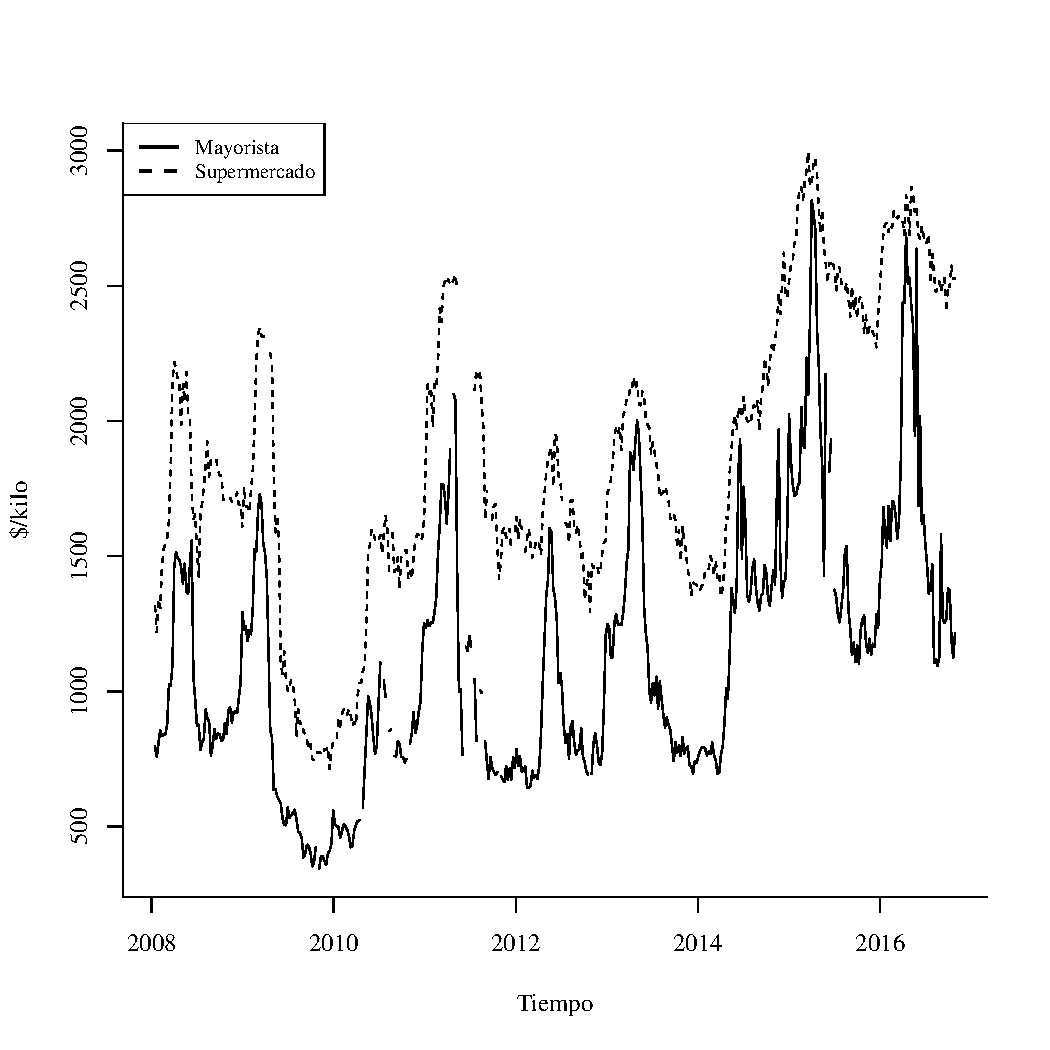
\includegraphics[width=6.5in,height=3.5in]{figure/fig-1-1} 

}

\caption[Evolución de precios del palta Hass de primera calidad,2008-2016]{Evolución de precios del palta Hass de primera calidad,2008-2016}\label{fig:fig-1}
\end{figure}


\end{knitrout}



\begin{knitrout}
\definecolor{shadecolor}{rgb}{0.969, 0.969, 0.969}\color{fgcolor}\begin{figure}[H]

{\centering 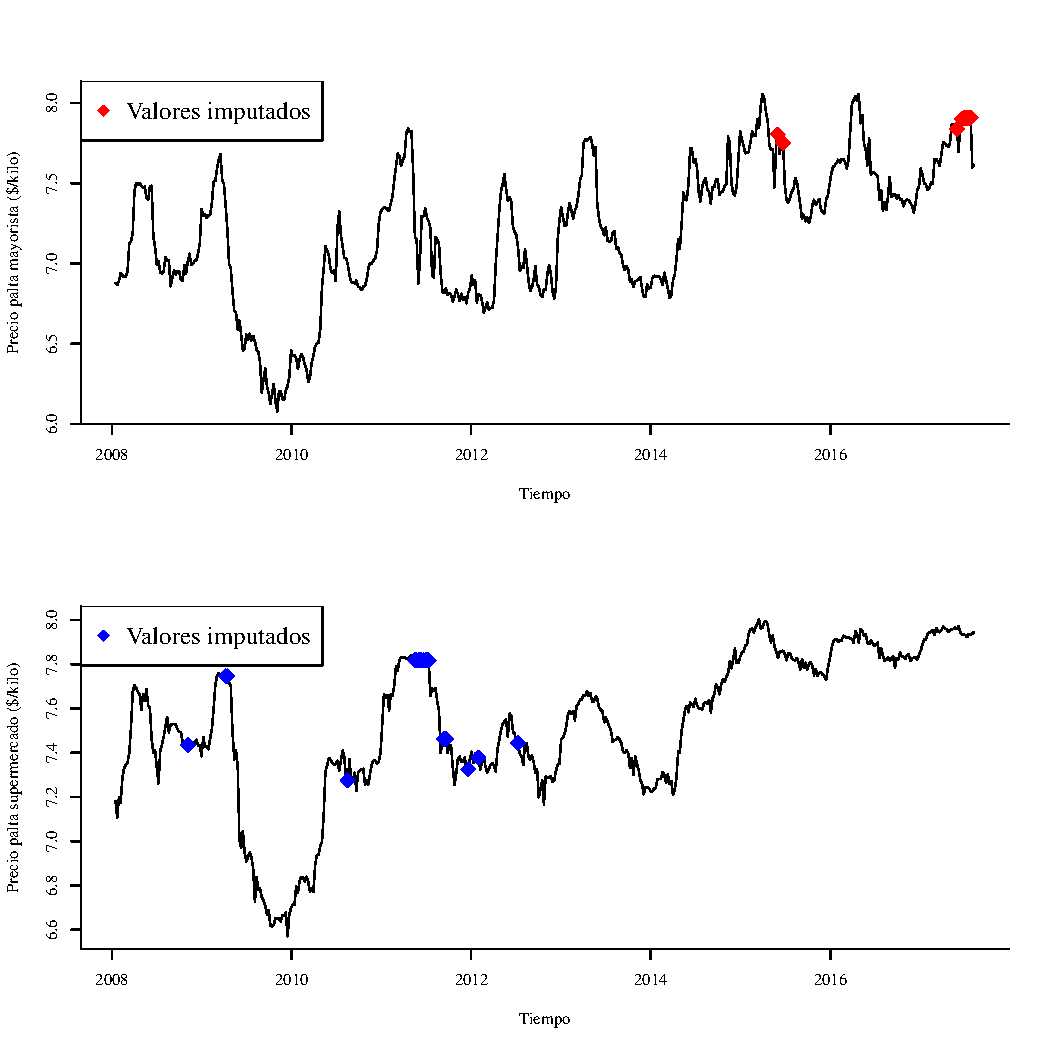
\includegraphics[width=6.5in,height=4.5in]{figure/fig-2-1} 

}

\caption[Imputación de valores perdidos a través del filtro de Kalman]{Imputación de valores perdidos a través del filtro de Kalman}\label{fig:fig-2}
\end{figure}


\end{knitrout}

\section{Análisis del orden de integración de las series}
\subsection{Análisis gráfico}

Para analizar el orden de integración de las series es de utilidad usar herramientas gráficas que entreguen cierta orientación sobre el comportamiento de las series antes de realizar un análisis formal a través de contrastes de hipótesis. 

Cabe señalar que, como un intento de estabilizar la varianza de las series, estas serán trabajadas en logaritmo.

\subsubsection{Análisis de las series en nivel}

En el caso del logaritmo de los precios mayoristas de la palta, puede apreciarse una media no constante, aunque lo mismo no es directamente apreciable  para la varianza. Por otro lado, su correlograma muestra autocorrelaciones significativas más allá de 52 períodos de rezago, lo que permite afirmar que el proceso tendría una memoria prolongada y que por tanto, no es estacionario (Véase figura \ref{fig5.1}).

Para el caso de la serie del logaritmo del precio de la palta en supermercados, se puede observar un comportamiento bastante similar. Es decir, una media que no es constante debido a una tendencia, cuya naturaleza se determina más adelante; y una memoria prolongada al observar el correlograma correspondiente (Véase figura \ref{fig5.2}).  


\begin{knitrout}
\definecolor{shadecolor}{rgb}{0.969, 0.969, 0.969}\color{fgcolor}\begin{figure}[H]

{\centering 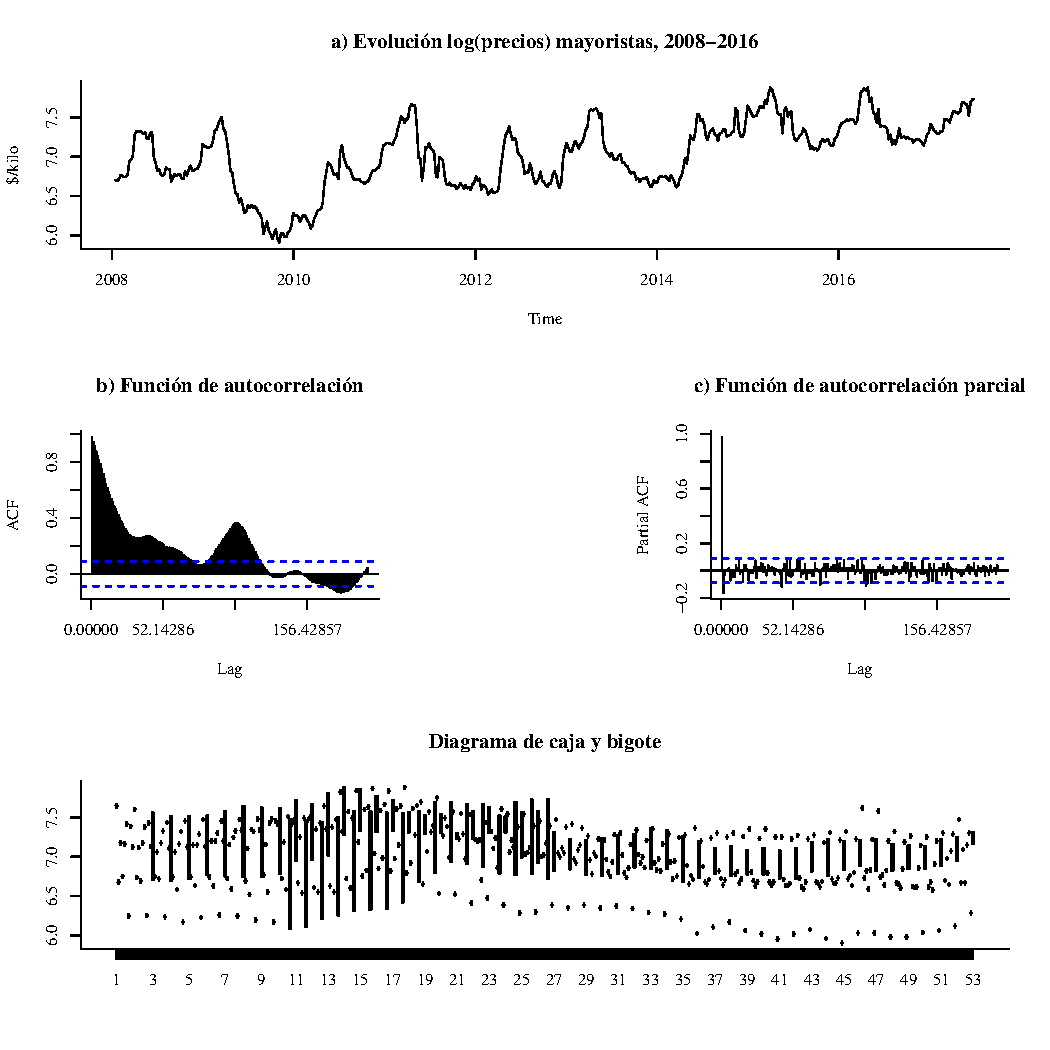
\includegraphics[width=4.5in,height=3.5in]{figure/fig-2_1-1} 

}

\caption{Evolución del logaritmo del precio mayorista de la palta, 2008-2016\label{fig5.1}}\label{fig:fig-2.1}
\end{figure}


\end{knitrout}


\begin{knitrout}
\definecolor{shadecolor}{rgb}{0.969, 0.969, 0.969}\color{fgcolor}\begin{figure}[H]

{\centering 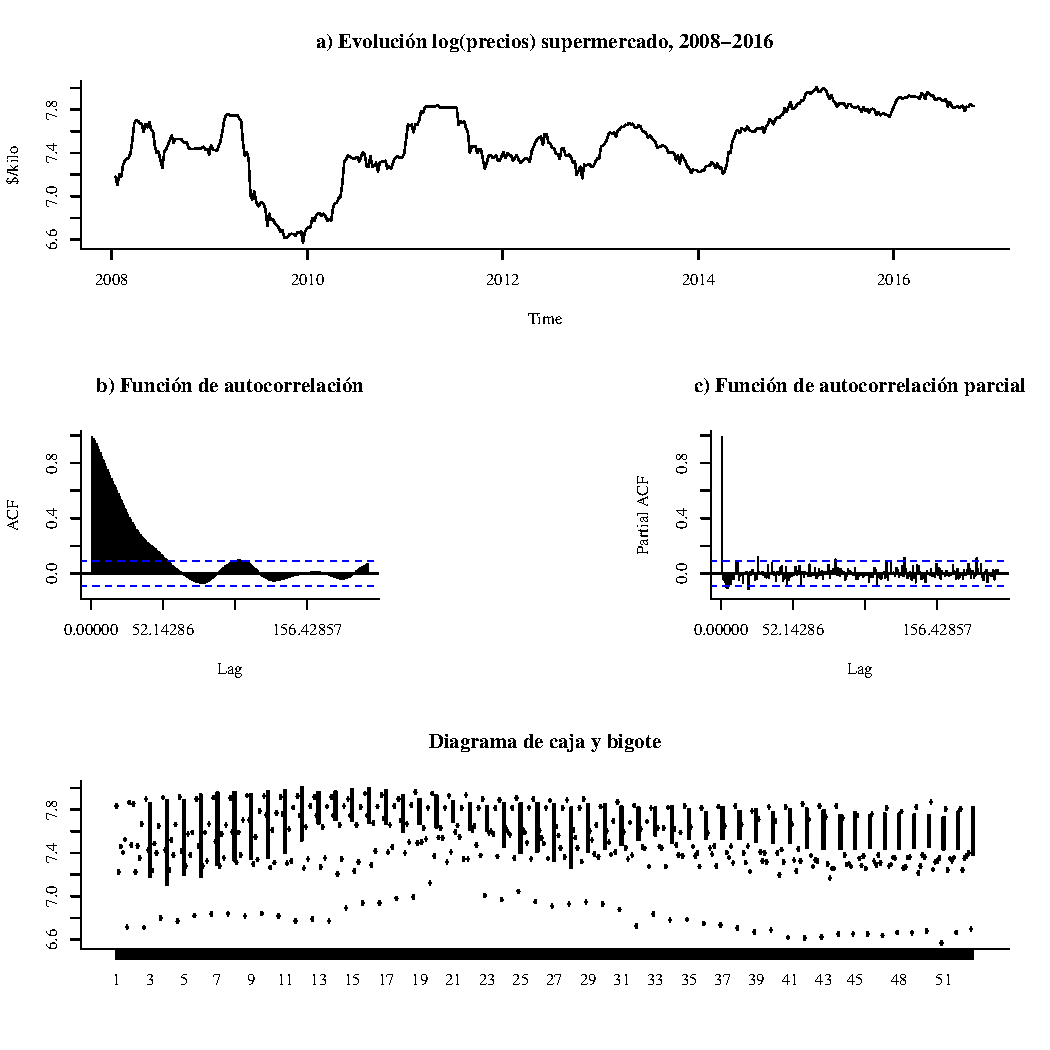
\includegraphics[width=4.5in,height=3.5in]{figure/fig-2_2-1} 

}

\caption{Evolución del logaritmo del precio en supermercado de la palta, 2008-2016\label{fig5.2}}\label{fig:fig-2.2}
\end{figure}


\end{knitrout}

\subsubsection{Análisis de las series en diferencias}

A continuación se procedió a diferenciar las series, pues existe la sospecha de la presencia de raíz unitaria en ambas, cuestión que será determinada más adelante.

Al analizar las figuras \ref{fig5.3} y \ref{fig5.4} se observan algunos rezagos significativos en el correlograma, lo que puede servir de orientación para determinar el orden de integración de las series. A pesar de lo anterior, se observa de todas maneras que el comportamiento de la varianza no es estable a lo largo del tiempo en ambos casos.  


\begin{knitrout}
\definecolor{shadecolor}{rgb}{0.969, 0.969, 0.969}\color{fgcolor}\begin{figure}[H]

{\centering 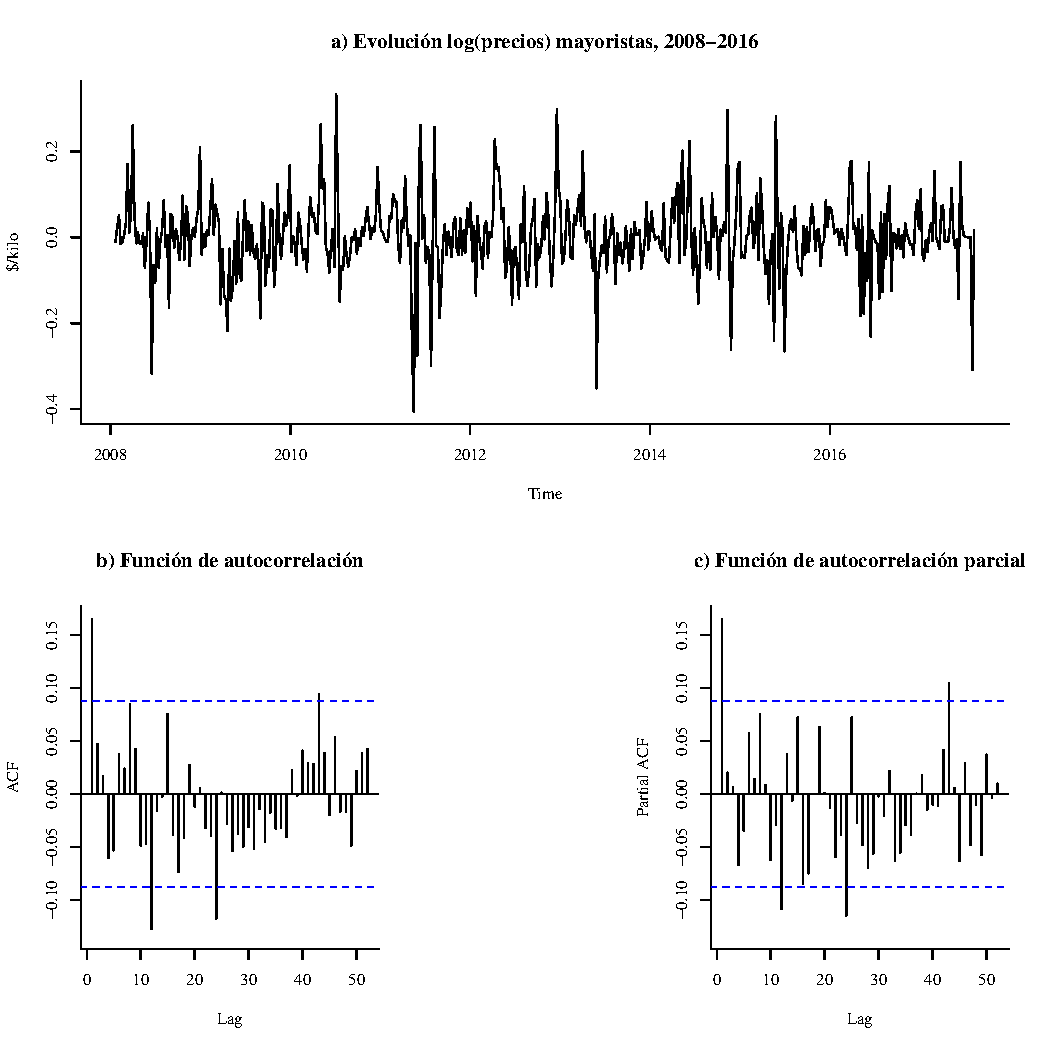
\includegraphics[width=4.5in,height=3.5in]{figure/fig-2_3-1} 

}

\caption{Evolución del logaritmo del precio mayorista de la palta, 2008-2016\label{fig5.3}}\label{fig:fig-2.3}
\end{figure}


\end{knitrout}


\begin{knitrout}
\definecolor{shadecolor}{rgb}{0.969, 0.969, 0.969}\color{fgcolor}\begin{figure}[H]

{\centering 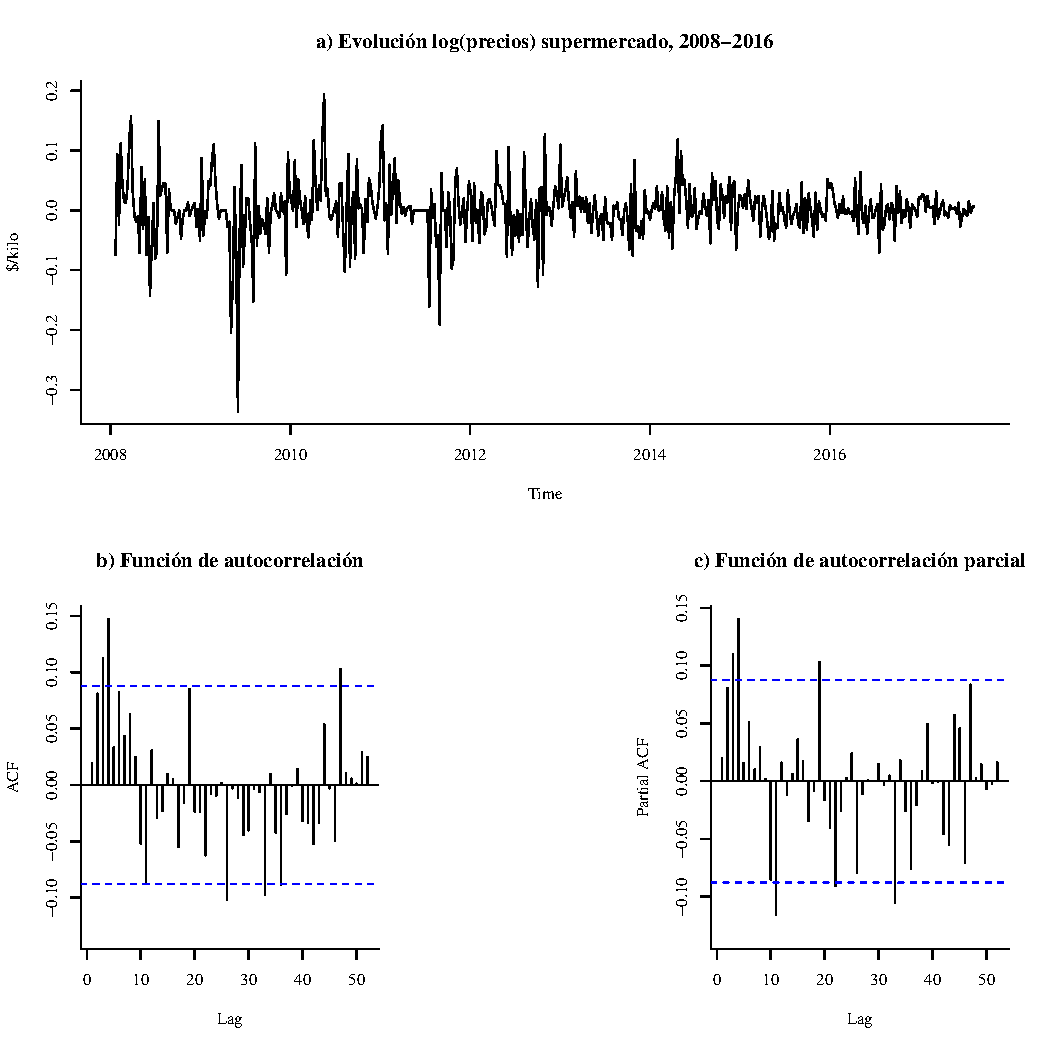
\includegraphics[width=4.5in,height=3.5in]{figure/fig-2_4-1} 

}

\caption{Evolución del logaritmo del precio en supermercado de la palta, 2008-2016\label{fig5.4}}\label{fig:fig-2.4}
\end{figure}


\end{knitrout}



\subsection{Contrastes de raíz unitaria}

\subsubsection{Análisis de las series originales}
Para determinar de manera formal la presencia de raíces unitarias en las series analizadas se procede a continuación a aplicar una serie de contrastes comúnmente utilizados en la literatura. 




A continuación se aplicará el contraste de Dickey-Fuller aumentado bajo el supuesto de que el proceso subyacente tiene drift y tendencia y bajo el supuesto de que sólo tiene drift. 

\begin{center}
\begin{table}[h]
\caption{Contraste de Dickey-Fuller aumentado (con drift)\label{tab:dickey1}}
\centering
\begin{threeparttable}
\begin{tabular}{@{}llllll@{}}
\toprule \\
\multicolumn{1}{l}{} & \multicolumn{2}{c}{Estimaciones} &
\multicolumn{3}{c}{Valores críticos} \\
\cmidrule(l){2-3} \cmidrule(l){4-6} \\
\multicolumn{1}{l}{} & \multicolumn{1}{c}{Mayorista$^{a}$} &
 \multicolumn{1}{c}{Supermercado$^{b}$} &
\multicolumn{1}{l}{90\%}&
\multicolumn{1}{l}{95\%}&
\multicolumn{1}{l}{99\%}
\\
\midrule
$\tau_{2} $  & -2.5725 &  -1.6393  & -2.57 & -2.87 & -3.44 \\
$\phi_{1} $  & 3.4095  &  1.6354   & 3.79 & 4.61 &  6.47\\
\bottomrule \\
\end{tabular}
\begin{tablenotes}
\small 
\item $^{a}$: Con un rezago, de acuerdo a criterio BIC. 
\item $^{b}$: Con un rezago, de acuerdo a criterio BIC. 
\end{tablenotes}
\end{threeparttable}
\end{table}
\end{center}



El cuadro \ref{tab:dickey1} muestra que la evidencia estadística provista por la realización de la serie es apenas suficiente para rechazar la hipótesis $\mathcal{H}_{0}: \rho = 1$ a un nivel de significancia de 10 \%. Por otro lado, la hipótesis $\mathcal{H}_{0}: (\alpha,\rho) = (0,1) $ no puede ser rechazada.

Con respecto a la serie de precios de supermercados la evidencia va en la misma dirección. 

De acuerdo a lo anterior, la serie no contendría una raíz unitaria. De todas maneras, es necesario formular otras representaciones del proceso, como bien podría ser incluir una tendencia determinista (a continuación) o utilizar otros contrastes. 

\begin{table}[h]
\centering
\begin{threeparttable}
\caption{Contraste de Dickey-Fuller aumentado (con tendencia)\label{tab:dickey2}}
\begin{tabular}{@{}llllll@{}}
\toprule
\multicolumn{1}{l}{} & \multicolumn{2}{c}{Estimaciones} &
\multicolumn{3}{c}{Valores críticos} \\
\cmidrule(l){2-3} \cmidrule(l){4-6} \\
\multicolumn{1}{l}{} & \multicolumn{1}{c}{Mayorista$^{a}$} &
 \multicolumn{1}{c}{Supermercado$^{b}$} &
\multicolumn{1}{l}{90\%}&
\multicolumn{1}{l}{95\%}&
\multicolumn{1}{l}{99\%}
\\
\midrule
$\tau_{3} $  & -3.4073 &  -2.1143  &  -3.13 & -3.42  &  -3.98 \\
$\phi_{2} $  & 3.9655  &  1.6848   &  4.05 &  4.71 &  6.15 \\
$\phi_{3} $  & 5.8467  &  2.2351   &  5.36 &  6.30 &  8.34 \\
\bottomrule
\end{tabular}
\begin{tablenotes}
\small 
\item $^{a}$: Con un rezago, de acuerdo a criterio BIC. 
\item $^{b}$: Con un rezago, de acuerdo a criterio BIC. 
\end{tablenotes}
\end{threeparttable}
\end{table}


El cuadro \ref{tab:dickey2} muestra que para el caso de la serie de precios mayoristas, la hipótesis $\mathcal{H}_{0}: \rho=1$ se rechaza a un nivel de significancia de $10\%$. Mientras que la hipótesis $\mathcal{H}_{0}: (\alpha, \beta, \rho)=(0,0,1)$  no muestra evidencia estadística suficiente para ser rechaza a los niveles de significancia propuestos. Por último, la hipótesis $\mathcal{H}_{0}: (\alpha, \beta,\rho)=(\alpha,0,1)$ puede ser rechazada sólo a un 10\% de significancia. 

Para el caso de la serie de precios de supermercado, la hipótesis $\mathcal{H}_{0}: \rho=1$ no puede ser rechazada a ninguno de los niveles de significancia propuestos. Mientras que el contraste tampoco provee información suficiente para rechazar $\mathcal{H}_{0}: (\alpha, \beta, \rho)=(0,0,1)$. Por último, la hipótesis $\mathcal{H}_{0}: (\alpha, \beta,\rho)=(\alpha,0,1)$ puede ser rechaza sólo a un 10\% de significancia. 

El resultado de este contraste es más bien contradictorio, pues no permite concluir que ambas series contengan una raíz unitaria, bajo los diferentes escenarios que sus hipótesis configuran. Queda la posibilidad entonces de que las series tengan un comportamiento estacionario en tendencia, situación que será abordada con el contraste KPSS. 

Los resultados del cuadro \ref{fig5.3}  muestran que para ambas series se rechaza la hipótesis de estacionariedad de la serie a nivel de significancia del 1\%. Razón por la cual se descarta la hipótesis de estacionariedad en tendencia. 

\begin{table}[h]
\centering
\begin{threeparttable}
\caption{Contraste KPSS (con tendencia determinista) \label{fig5.3}}
\begin{tabular}{@{}lrllll@{}}
\toprule
\multicolumn{1}{l}{} & \multicolumn{2}{c}{Estadístico} &
\multicolumn{3}{c}{Valores críticos} \\
\cmidrule(l){2-3} \cmidrule(l){4-6} \\
\multicolumn{1}{l}{$\mathcal{H}_0$} & \multicolumn{1}{c}{Mayorista$^{a}$} &
 \multicolumn{1}{c}{Supermercado$^{b}$} &
\multicolumn{1}{l}{90\%}&
\multicolumn{1}{l}{95\%}&
\multicolumn{1}{l}{99\%}
\\
\midrule
$\tau_{3} $  & 0.2405 &  0.3223 & 0.119 & 0.146 & 0.216 \\
\bottomrule
\end{tabular}
\label{tab-6}
\begin{tablenotes}
\small 
\item $^{a}$: Con cinco rezagos de acuerdo a la siguiente regla $\root 4 \of {4 \times (n/100)}$. 
\item $^{b}$: Con cinco rezagos de acuerdo a la siguiente regla $\root 4 \of {4 \times (n/100)}$. 
\end{tablenotes}
\end{threeparttable}
\end{table}

Por otro lado, los resultados del cuadro \ref{fig5.4} indican que la hipótesis de estacionariedad en niveles se rechaza fuertemente en ambos casos. 

\begin{table}[h]
\centering
\begin{threeparttable}
\caption{Contraste KPSS (sin tendencia determinista) \label{fig5.4}}
\begin{tabular}{@{}lrllll@{}}
\toprule
\multicolumn{1}{l}{} & \multicolumn{2}{c}{Estadístico} &
\multicolumn{3}{c}{Valores críticos} \\
\cmidrule(l){2-3} \cmidrule(l){4-6} \\
\multicolumn{1}{l}{$\mathcal{H}_0$} & \multicolumn{1}{c}{Mayorista$^{a}$} &
 \multicolumn{1}{c}{Supermercado$^{b}$} &
\multicolumn{1}{l}{90\%}&
\multicolumn{1}{l}{95\%}&
\multicolumn{1}{l}{99\%}
\\
\midrule
$\tau_{3} $  & 3.5537 &  3.8913 & 0.347 & 0.463 & 0.739 \\
\bottomrule
\end{tabular}
\label{tab-7}
\begin{tablenotes}
\small 
\item $^{a}$: Con cinco rezagos de acuerdo a la siguiente regla $\root 4 \of {4 \times (n/100)}$. 
\item $^{b}$: Con cinco rezagos de acuerdo a la siguiente regla $\root 4 \of {4 \times (n/100)}$. 
\end{tablenotes}
\end{threeparttable}
\end{table}

El contraste de Phillips Perron indica que no se puede rechazar la hipótesis de raíz unitaria para ambas series. 



\begin{table}[h]
\centering
\begin{threeparttable}
\caption{Contraste Phillips \& Perron$^{a}$ (con tendencia determinista)\label{tab:pperron1}}
\begin{tabular}{@{}llllll@{}}
\toprule
\multicolumn{1}{c}{} &
\multicolumn{1}{l}{Mayorista} &
\multicolumn{1}{l}{Supermercado} & 
90\% & 95\% & 99\% 
\\
\cmidrule(l){2-2} \cmidrule(l){3-3} \cmidrule(l){4-6} \\
$Z(t_{\hat{\alpha}})$ &-22.1367 & -11.958 & -3.13 & -3.42 & -3.98 \\ 
$Z(t_{\hat{\mu}})$    &  1.5224 & 1.0702  &  4.04 & 4.71  & 6.15  \\ 
$Z(t_{\hat{\beta}})$  &  2.2482 & 1.6792  &  5.63 & 6.30  & 8.34 \\
\bottomrule
\end{tabular}
\label{tab-4}
\begin{tablenotes}
\small 
\item $^{a}$: Con cinco rezagos de acuerdo a la siguiente regla $\root 4 \of {4 \times (n/100)}$. 
\end{tablenotes}
\end{threeparttable}
\end{table}

El cuadro \ref{tab:pperron1} muestra que el contraste rechaza la hipótesis de raíz unitaria, aunque no permite identificar con claridad la estructura de los términos deterministas. 





\begin{table}[h]
\centering
\begin{threeparttable}
\caption{Contraste Phillips \& Perron$^{a}$ (con tendencia determinista) \label{tab:pperron2}}
\begin{tabular}{@{}llllll@{}}
\toprule
\multicolumn{1}{c}{} &
\multicolumn{1}{l}{Mayorista} & 
\multicolumn{1}{l}{Supermercado} & 
90\% & 95\% & 99\% \\ 
\\
\cmidrule(l){2-2} \cmidrule(l){3-3} \cmidrule(l){4-6} \\
$Z(t_{\hat{\alpha}})$ & -13.3185 & -6.8276 &  -2.57 & -2.87 & -3.44 \\
$Z(t_{\hat{\mu}})$ & 2.5034 & 1.8389 & 3.79 & 4.61 & 6.47 \\
\bottomrule
\end{tabular}
\label{tab-5}
\begin{tablenotes}
\small 
\item $^{a}$: Con cinco rezagos de acuerdo a la siguiente regla $\root 4 \of {4 \times (n/100)}$. 
\end{tablenotes}
\end{threeparttable}
\end{table}

Al observar el cuadro \ref{tab:pperron2} queda de manifiesto el rechazo de la hipótesis de raíz unitaria, aunque por cierto, no se puede afirmar con exactitud el comportamiento de los términos deterministas. 



Hecho lo anterior, se procede a aplicar el contraste ERS, utilizando en primer lugar un modelo con constante y tendencia deteminista. El cuadro \ref{fig5.5} muestra que para el caso de los mayoristas no se puede rechazar la hipótesis nula de raíz unitaria para ninguno de los niveles de significancia prescritos, mientras que para el caso de la serie supermercado dicha hipótesis se rechaza al menos al 5\%.  

\begin{table}[h]
\centering
\begin{threeparttable}
\caption{Contraste de Elliot, Rothenberg \& Stock (con tendencia determinista)\label{fig5.5}}
\begin{tabular}{@{}lrllll@{}}
\toprule
\multicolumn{1}{l}{} & \multicolumn{2}{c}{Estadístico} &
\multicolumn{3}{c}{Valores críticos} \\
\cmidrule(l){2-3} \cmidrule(l){4-6} \\
\multicolumn{1}{l}{} & \multicolumn{1}{c}{Mayorista$^{a}$} &
 \multicolumn{1}{c}{Supermercado$^{b}$} &
\multicolumn{1}{l}{90\%}&
\multicolumn{1}{l}{95\%}&
\multicolumn{1}{l}{99\%}
\\
\midrule
  & 3.8715 &  10.0306 & 6.89 & 5.62 & 3.96 \\
\bottomrule
\end{tabular}
\label{tab-8}
\begin{tablenotes}
\small 
\item $^{a}$: Con un rezago, de acuerdo a criterio BIC. 
\item $^{b}$: Con un rezago, de acuerdo a criterio BIC. 
\end{tablenotes}
\end{threeparttable}
\end{table}

El cuadro \ref{fig5.6}

\begin{table}[h]
\centering
\begin{threeparttable}
\caption{Contraste de Elliot, Rothenberg \& Stock (con constante)\label{fig5.6}}
\begin{tabular}{@{}lrllll@{}}
\toprule
\multicolumn{1}{l}{} & \multicolumn{2}{c}{Estadístico} &
\multicolumn{3}{c}{Valores críticos} \\
\cmidrule(l){2-3} \cmidrule(l){4-6} \\
\multicolumn{1}{l}{} & \multicolumn{1}{c}{Mayorista$^{a}$} &
 \multicolumn{1}{c}{Supermercado$^{b}$} &
\multicolumn{1}{l}{90\%}&
\multicolumn{1}{l}{95\%}&
\multicolumn{1}{l}{99\%}
\\
\midrule
  & 3.0049 &  12.0408 & 4.48 & 3.26 & 1.99 \\
\bottomrule
\end{tabular}
\label{tab-9}
\begin{tablenotes}
\small 
\item $^{a}$: Con un rezago, de acuerdo a criterio BIC. 
\item $^{b}$: Con un rezago, de acuerdo a criterio BIC. 
\end{tablenotes}
\end{threeparttable}
\end{table}








\subsubsection{Análisis de las series en diferencias}

Una vez establecida la presencia de raíces unitarias en las series, se procederá a aplicar los contrastes nuevamente para las series en diferencias




\begin{center}
\begin{table}[h]
\caption{Contraste de Dickey-Fuller aumentado (sin drift y tendencia)\label{tab:dickey1}}
\centering
\begin{threeparttable}
\begin{tabular}{@{}llllll@{}}
\toprule \\
\multicolumn{1}{l}{} & \multicolumn{2}{c}{Estimaciones} &
\multicolumn{3}{c}{Valores críticos} \\
\cmidrule(l){2-3} \cmidrule(l){4-6} \\
\multicolumn{1}{l}{} & \multicolumn{1}{c}{Mayorista$^{a}$} &
 \multicolumn{1}{c}{Supermercado$^{b}$} &
\multicolumn{1}{l}{90\%}&
\multicolumn{1}{l}{95\%}&
\multicolumn{1}{l}{99\%}
\\
\midrule
$\tau_{3} $  &  -14.0093 &  -14.3253  & -1.62 & -1.95 & -2.58 \\
\bottomrule \\
\end{tabular}
\begin{tablenotes}
\small 
\item $^{a}$: Con un rezago, de acuerdo a criterio BIC. 
\item $^{b}$: Con un rezago, de acuerdo a criterio BIC. 
\end{tablenotes}
\end{threeparttable}
\end{table}
\end{center}



Por otro lado, los resultados del cuadro \ref{fig5.4} indican que la hipótesis de estacionariedad en niveles se rechaza fuertemente en ambos casos. 



\begin{table}[h]
\centering
\begin{threeparttable}
\caption{Contraste KPSS (sin tendencia determinista) \label{tab5.4}}
\begin{tabular}{@{}lrllll@{}}
\toprule
\multicolumn{1}{l}{} & \multicolumn{2}{c}{Estadístico} &
\multicolumn{3}{c}{Valores críticos} \\
\cmidrule(l){2-3} \cmidrule(l){4-6} \\
\multicolumn{1}{l}{$\mathcal{H}_0$} & \multicolumn{1}{c}{Mayorista$^{a}$} &
 \multicolumn{1}{c}{Supermercado$^{b}$} &
\multicolumn{1}{l}{90\%}&
\multicolumn{1}{l}{95\%}&
\multicolumn{1}{l}{99\%}
\\
\midrule
$\tau_{3} $  & 0.0236 &  0.0433 & 0.347 & 0.463 & 0.739 \\
\bottomrule
\end{tabular}
\label{tab-7}
\begin{tablenotes}
\small 
\item $^{a}$: Con cinco rezagos de acuerdo a la siguiente regla $\root 4 \of {4 \times (n/100)}$. 
\item $^{b}$: Con cinco rezagos de acuerdo a la siguiente regla $\root 4 \of {4 \times (n/100)}$. 
\end{tablenotes}
\end{threeparttable}
\end{table}

El contraste KPSS muestra claramente como, ahora que la serie ha sido diferenciada, no se puede rechazar la hipótesis nula de estacionariedad. 

El contraste de Phillips Perron indica que no se puede rechazar la hipótesis de raíz unitaria para ambas series. 



\begin{table}[h]
\centering
\begin{threeparttable}
\caption{Contraste Phillips \& Perron$^{a}$ (con tendencia determinista)\label{tab:pperron1}}
\begin{tabular}{@{}llllll@{}}
\toprule
\multicolumn{1}{c}{} &
\multicolumn{1}{l}{Mayorista} &
\multicolumn{1}{l}{Supermercado} & 
90\% & 95\% & 99\% 
\\
\cmidrule(l){2-2} \cmidrule(l){3-3} \cmidrule(l){4-6} \\
$Z(t_{\hat{\alpha}})$ &-411.6423 & -571.565 & -3.13 & -3.42 & -3.98 \\ 
$Z(t_{\hat{\mu}})$    &  0.3197 & 0.7824  &  4.04 & 4.71  & 6.15  \\ 
\bottomrule
\end{tabular}
\label{tab-4}
\begin{tablenotes}
\small 
\item $^{a}$: Con un rezago de acuerdo a la siguiente regla $\root 4 \of {4 \times (n/100)}$. 
\end{tablenotes}
\end{threeparttable}
\end{table}

El cuadro \ref{tab:pperron1} muestra que el contraste rechaza la hipótesis de raíz unitaria, y que como es de esperar, la serie no contiene término constante. 





\begin{table}[h]
\centering
\begin{threeparttable}
\caption{Contraste Phillips \& Perron$^{a}$ (con tendencia determinista) \label{tab:pperron2}}
\begin{tabular}{@{}llllll@{}}
\toprule
\multicolumn{1}{c}{} &
\multicolumn{1}{l}{Mayorista} & 
\multicolumn{1}{l}{Supermercado} & 
90\% & 95\% & 99\% \\ 
\\
\cmidrule(l){2-2} \cmidrule(l){3-3} \cmidrule(l){4-6} \\
$Z(t_{\hat{\alpha}})$ & -13.3185 & -6.8276 &  -2.57 & -2.87 & -3.44 \\
$Z(t_{\hat{\mu}})$ & 2.5034 & 1.8389 & 3.79 & 4.61 & 6.47 \\
\bottomrule
\end{tabular}
\label{tab-5}
\begin{tablenotes}
\small 
\item $^{a}$: Con cinco rezagos de acuerdo a la siguiente regla $\root 4 \of {4 \times (n/100)}$. 
\end{tablenotes}
\end{threeparttable}
\end{table}

Al observar el cuadro \ref{tab:pperron2} queda de manifiesto el rechazo de la hipótesis de raíz unitaria, aunque por cierto, no se puede afirmar con exactitud el comportamiento de los términos deterministas. 



Hecho lo anterior, se procede a aplicar el contraste ERS, utilizando en primer lugar un modelo con constante y tendencia deteminista. El cuadro \ref{fig5.5} muestra que para el caso de los mayoristas no se puede rechazar la hipótesis nula de raíz unitaria para ninguno de los niveles de significancia prescritos, mientras que para el caso de la serie supermercado dicha hipótesis se rechaza al menos al 5\%.  

\begin{table}[h]
\centering
\begin{threeparttable}
\caption{Contraste de Elliot, Rothenberg \& Stock (con tendencia determinista)\label{fig5.5}}
\begin{tabular}{@{}lrllll@{}}
\toprule
\multicolumn{1}{l}{} & \multicolumn{2}{c}{Estadístico} &
\multicolumn{3}{c}{Valores críticos} \\
\cmidrule(l){2-3} \cmidrule(l){4-6} \\
\multicolumn{1}{l}{} & \multicolumn{1}{c}{Mayorista$^{a}$} &
 \multicolumn{1}{c}{Supermercado$^{b}$} &
\multicolumn{1}{l}{90\%}&
\multicolumn{1}{l}{95\%}&
\multicolumn{1}{l}{99\%}
\\
\midrule
  & 3.8715 &  10.0306 & 6.89 & 5.62 & 3.96 \\
\bottomrule
\end{tabular}
\label{tab-8}
\begin{tablenotes}
\small 
\item $^{a}$: Con un rezago, de acuerdo a criterio BIC. 
\item $^{b}$: Con un rezago, de acuerdo a criterio BIC. 
\end{tablenotes}
\end{threeparttable}
\end{table}

El cuadro \ref{fig5.6}

\begin{table}[h]
\centering
\begin{threeparttable}
\caption{Contraste de Elliot, Rothenberg \& Stock (con constante)\label{fig5.6}}
\begin{tabular}{@{}lrllll@{}}
\toprule
\multicolumn{1}{l}{} & \multicolumn{2}{c}{Estadístico} &
\multicolumn{3}{c}{Valores críticos} \\
\cmidrule(l){2-3} \cmidrule(l){4-6} \\
\multicolumn{1}{l}{} & \multicolumn{1}{c}{Mayorista$^{a}$} &
 \multicolumn{1}{c}{Supermercado$^{b}$} &
\multicolumn{1}{l}{90\%}&
\multicolumn{1}{l}{95\%}&
\multicolumn{1}{l}{99\%}
\\
\midrule
  & 3.0049 &  12.0408 & 4.48 & 3.26 & 1.99 \\
\bottomrule
\end{tabular}
\label{tab-9}
\begin{tablenotes}
\small 
\item $^{a}$: Con un rezago, de acuerdo a criterio BIC. 
\item $^{b}$: Con un rezago, de acuerdo a criterio BIC. 
\end{tablenotes}
\end{threeparttable}
\end{table}




A partir del análisis recién expuesto, se puede concluir que ambas series al ser diferenciadas tienen un comportamiento estacionario. De forma tal que ambas series son I(1).

De esta forma, se procederá a determinar si la tendencia estocástica es compartida a través de un análisis de cointegración. 

\section{Determinación del rango de cointegración y estimación del modelo del modelo lineal de corrección del error}

En este apartado se utiliza principalmente con el paquete \texttt{vars} (Pfaff, 2008). 



Antes de la determinación del rango de cointegración del proceso, es necesario tener en cuenta que el uso del contraste de cointegración de Johansen que se utilizará para dichos fines es sensible a la especificación del modelo vectorial de corrección del equilibrio que subyace. Para la especificación de dicho modelo se recurrió a diferentes criterios. 

De manera similar a como señalan Ben Kaabia \& Gil (2008), se observa que al realizar los contrastes univariantes de raíz unitaria, no se rechaza la existencia de una raíz unitaria en torno a una constante no nula. Así también, al realizar los mismos contrastes para las series en primeras diferencias, las series resultaron estacionarias. Por último, en términos económicos, la presencia de una constante indica que existe una diferencia de escala entre los precios mayoristas y detallistas. 

El número de rezagos a incluir en el modelo se determinó con el objetivo de prevenir problemas de autocorrelación. De esta manera, se estimó el modelo secuencialmente utilizando entre 2 y  12 rezagos y se calculó el estadístico de Ljung-Box multivariado para los residuos rezagados entre el orden mínimo posible y aquellos de orden 52. Los p-valores correspondientes a cada uno de los contrastes están resumidos en la figura \ref{fig5.6}. De esta manera, se aprecia que la hipótesis nula de independencia no se puede rechazar a un nivel de significancia de 5\% en la mayoría de los casos para el modelo con ocho términos rezagados. 

\begin{knitrout}
\definecolor{shadecolor}{rgb}{0.969, 0.969, 0.969}\color{fgcolor}\begin{figure}[H]

{\centering 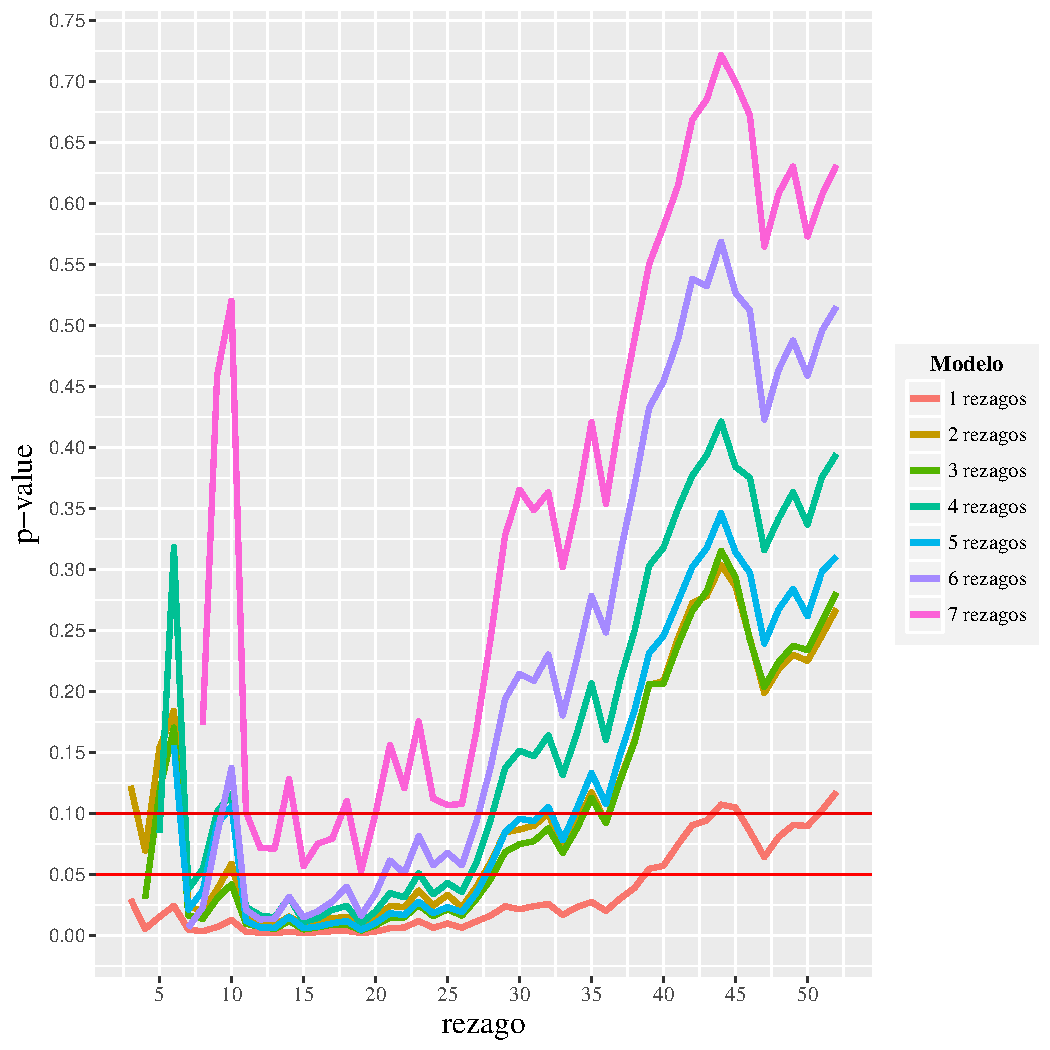
\includegraphics[width=5in,height=3.5in]{figure/unnamed-chunk-18-1} 

}

\caption{Número de Rezagos para el contraste de Independencia\label{fig5.6}}\label{fig:unnamed-chunk-18}
\end{figure}


\end{knitrout}

De esta forma, el modelo definitivo a estimar resultó ser el siguiente: 

\begin{equation}
\Delta \mathbf{y}_{t} = \boldsymbol{\Pi}\mathbf{y}_{t-1}+\sum_{i=1}^{8}\boldsymbol{\Gamma_{i}}\mathbf{y}_{t-i}+\boldsymbol{\varepsilon}_{t}
\end{equation}

Entonces, definido el número de rezagos a utilizar y la estructura del vector cointegrante, se procedió a aplicar el contraste de cointegración de Johansen, cuyos resultados pueden apreciarse en los cuadros \ref{tab5.15} y \ref{tab5.16}






\begin{table}[h]
\caption{Contraste de la \textit{la traza} de cointegración de Johansen\label{tab5.15}}
\begin{center}
\begin{tabular}{@{}lrllll@{}}
\toprule
\multicolumn{1}{l}{} & \multicolumn{2}{c}{Estadístico} &
\multicolumn{3}{c}{Valores críticos} \\
\cmidrule(l){2-3} \cmidrule(l){4-6} \\
\multicolumn{1}{l}{$\mathcal{H}_0$} & \multicolumn{2}{c}{$p = 8$} &
\multicolumn{1}{l}{90\%}&
\multicolumn{1}{l}{95\%}&
\multicolumn{1}{l}{99\%}
\\
\midrule
$r \leq 1$  & \multicolumn{2}{c}{5.82}  & 7.52 & 9.24 & 12.97\\
$r = 0$     & \multicolumn{2}{c}{ 36.63}  & 17.85 & 19.96 & 24.60\\
\bottomrule
\end{tabular}
\end{center}
\label{tab-10}
\end{table}

En el cuadro \ref{tab5.15} se observa el rechazo de la hipótesis $\mathcal{H}_{0}: = 0$ lo que descarta que la especificación adecuada sea un modelo VAR en niveles. Por otro lado, la hipótesis nula $\mathcal{H}_{0}\leq 1$ no puede rechazarse. 


\begin{table}[h]
\caption{Contraste del \textit{máximo autovalor} de cointegración de Johansen\label{tab5.16}}
\begin{center}
\begin{tabular}{@{}lrllll@{}}
\toprule
\multicolumn{1}{l}{} & \multicolumn{2}{c}{Estadístico} & \multicolumn{3}{c}{Valores críticos} \\
\cmidrule(l){2-3} \cmidrule(l){4-6} \\
\multicolumn{1}{l}{$\mathcal{H}_0$} & \multicolumn{2}{c}{$p = 8$} &
\multicolumn{1}{l}{90\%}&
\multicolumn{1}{l}{95\%}&
\multicolumn{1}{l}{99\%}
\\
\midrule
$r \leq 1$ & \multicolumn{2}{c}{5.82} & 7.52 & 9.24 & 12.97 \\
$r = 0$ & \multicolumn{2}{c}{30.82} & 13.75 & 15.67 & 20.20 \\
\bottomrule
\end{tabular}
\end{center}
\label{tab-11}
\end{table}

Al realizar la prueba de acuerdo al máximo autovalor, se observa el mismo resultado. 

De esta manera, el modelo puede especificarse como 

\begin{equation}
 \Delta\mathbf{y}_{t} = \boldsymbol{\alpha \beta}^{'}\left[\begin{array}{c}1 \\ \mathbf{y}_{t-1}\end{array}\right]+\sum_{i=1}^{8}\boldsymbol{\Gamma}_{i}\Delta\mathbf{y}_{t-i}+\boldsymbol{\varepsilon}_{t}
\end{equation}

Donde $\boldsymbol{\alpha}=\left[\begin{array}{c} \alpha_{1} \\ \alpha_{2} \\ \alpha_{3} \end{array}\right]$ y $\boldsymbol{\beta}^{'} = \left[\begin{array}{ccc} \beta_{1} & \beta_{2} & \beta_{3} \end{array}\right]$


\begin{knitrout}
\definecolor{shadecolor}{rgb}{0.969, 0.969, 0.969}\color{fgcolor}\begin{kframe}
\begin{verbatim}
## [1] 0.5149079
\end{verbatim}
\end{kframe}
\end{knitrout}



\begin{table}[h]
\centering
\begin{threeparttable}
\caption{Contraste de Elliot, Rothenberg \& Stock (con constante)\label{fig5.6}}
\begin{tabular}{@{}lll@{}}
\toprule
 & $\Delta \text{mayorista}_{t} $ & $\Delta \text{supermerado}_{t}$ \\ 
 \midrule 
 $\text{corrección del error}$ & -0.146592   &  0.027821 \\     
$\Delta$mayorista$_{t-1}$   &   0.065270 &   0.095569  \\   
$\Delta$supermercado$_{t-1}$  & 0.333719  &  -0.095055 \\     
$\Delta$mayorista$_{t-2}$  & -0.075599  &   0.112612  \\   
$\Delta$supermercado$_{t-1}$  & 0.296286  &  -0.042207 \\     
$\Delta$mayorista$_{t-3}$ &  -0.095907  & 0.063245     \\
$\Delta$supermercado$_{t-3}$  & 0.198395  &   0.006723  \\   
$\Delta$mayorista$_{t-4}$   &  -0.174854  &   0.046165 \\     
$\Delta$supermercado$_{t-4}$  & 0.212239  &   0.053372  \\   
$\Delta$mayorista$_{t-5}$   &  -0.175601  &  -0.004331 \\     
$\Delta$supermercado$_{t-5}$  & 0.167277  &  -0.057114  \\   
$\Delta$mayorista$_{t-6}$   & -0.064872   &  0.068671 \\     
$\Delta$supermercado$_{t-1}$  & 0.148495  &  -0.011887 \\     
$\Delta$mayorista$_{t-7}$   &  -0.122949  &   0.101965 \\     
$\Delta$supermercado$_{t-7}$  & 0.332634  &  -0.042574  \\   
$\Delta$mayorista$_{t-8}$   &  -0.067370  &   0.009668  \\   
$\Delta$supermercado$_{t-1}$  & 0.107484  &  -0.033937  \\ 
\bottomrule
\end{tabular}
\label{tab-9}
\begin{tablenotes}
\small 
\item $^{a}$: Con un rezago, de acuerdo a criterio BIC. 
\item $^{b}$: Con un rezago, de acuerdo a criterio BIC. 
\end{tablenotes}
\end{threeparttable}
\end{table}






\begin{knitrout}
\definecolor{shadecolor}{rgb}{0.969, 0.969, 0.969}\color{fgcolor}\begin{figure}[H]

{\centering 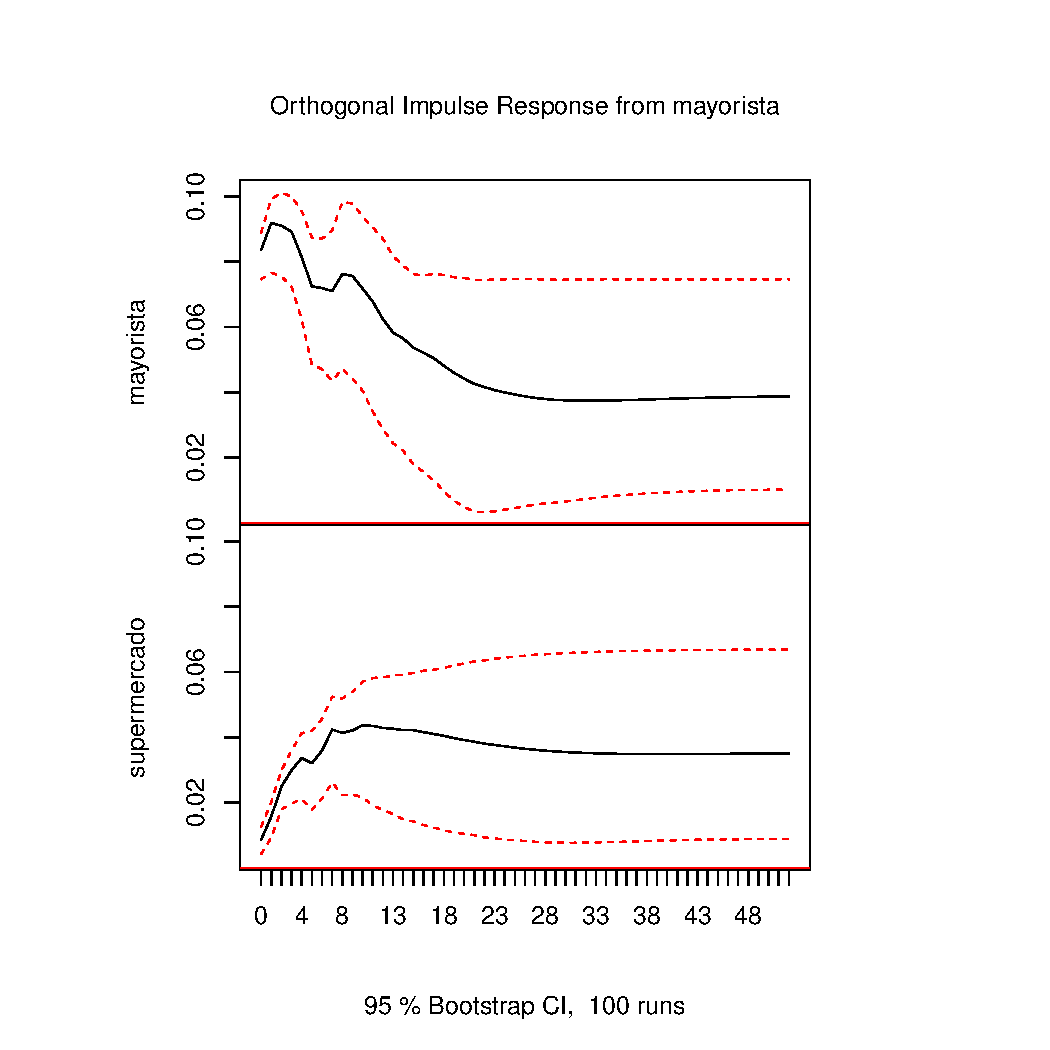
\includegraphics[width=4.5in,height=3.5in]{figure/graph5_6-1} 

}

\caption{Función ortogonal de impulso respuesta\label{graph5.6}}\label{fig:graph5.61}
\end{figure}

\begin{figure}[H]

{\centering 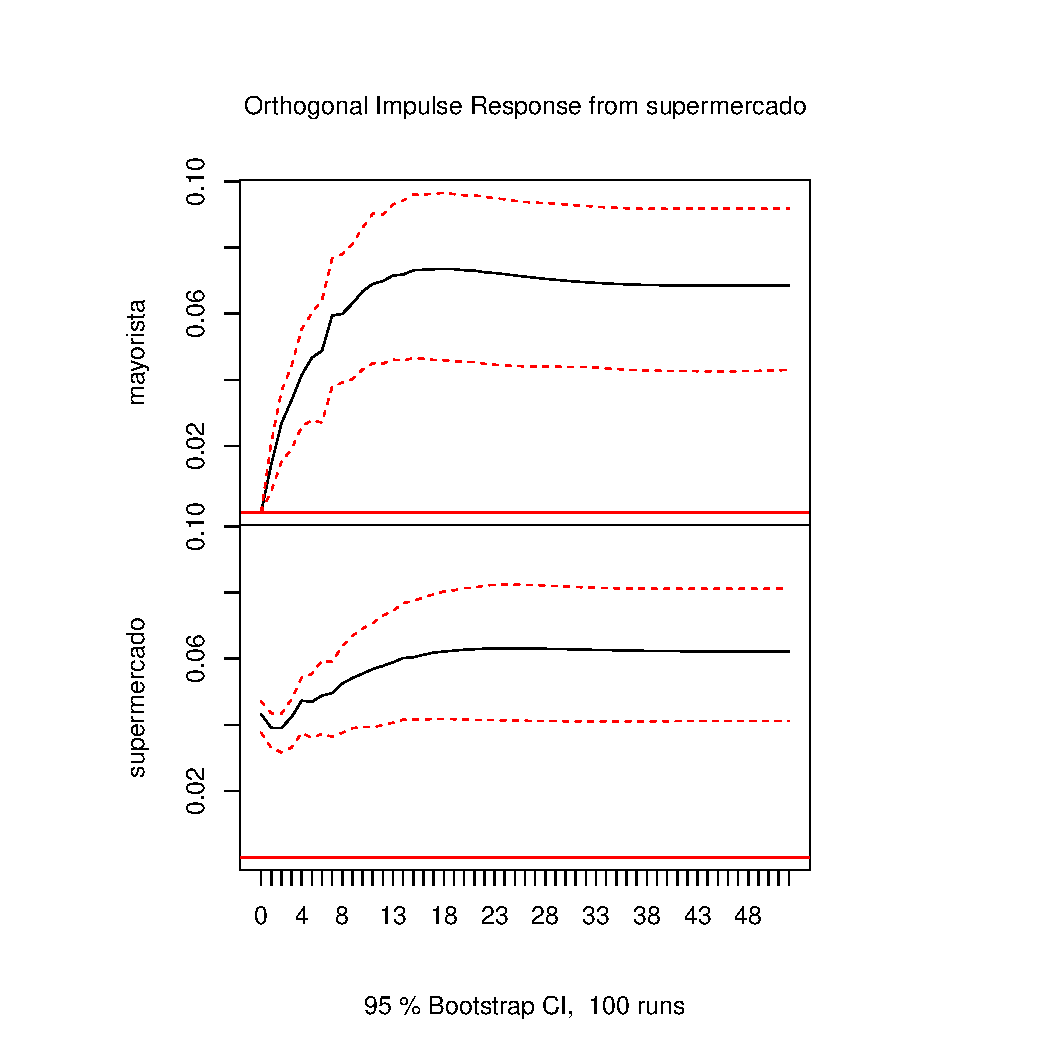
\includegraphics[width=4.5in,height=3.5in]{figure/graph5_6-2} 

}

\caption{Función ortogonal de impulso respuesta\label{graph5.6}}\label{fig:graph5.62}
\end{figure}


\end{knitrout}

\begin{knitrout}
\definecolor{shadecolor}{rgb}{0.969, 0.969, 0.969}\color{fgcolor}\begin{figure}[H]

{\centering 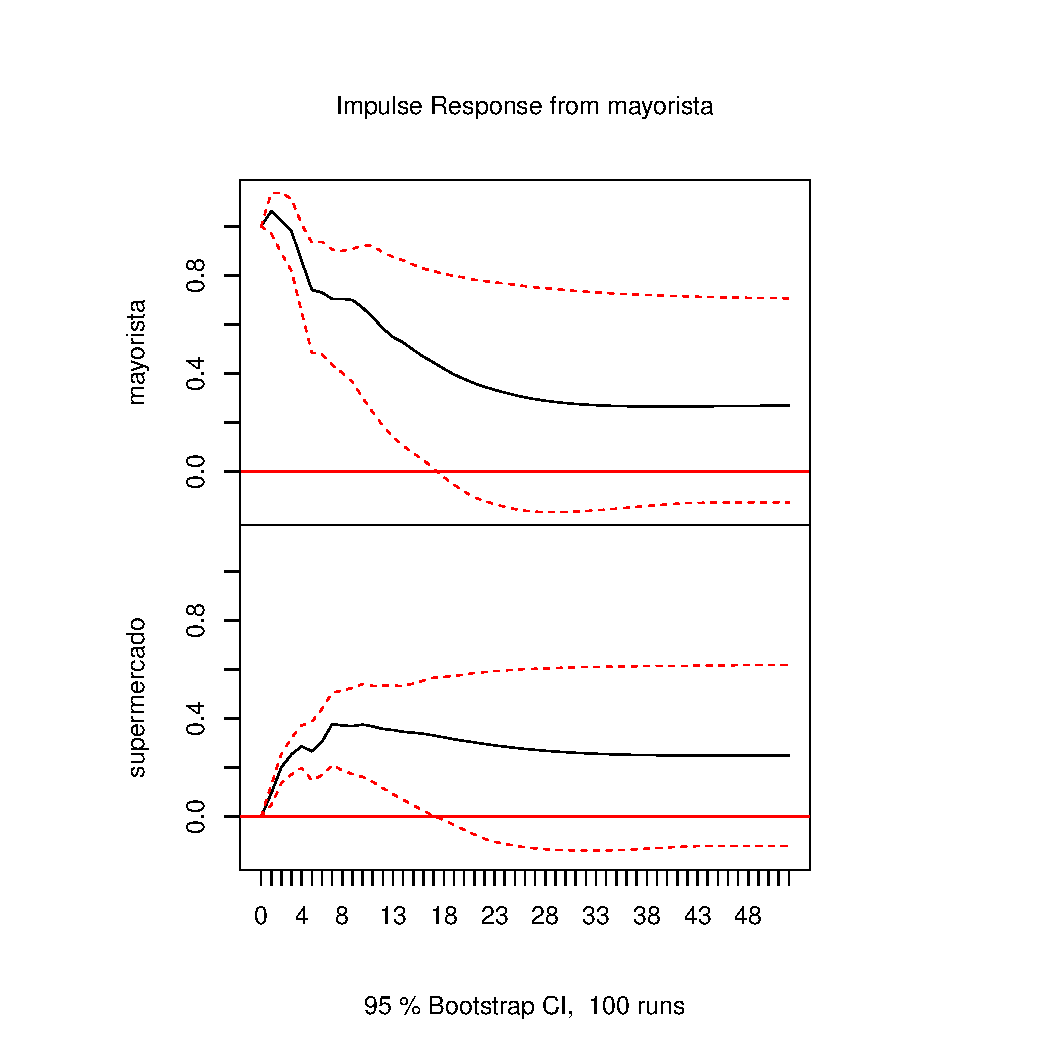
\includegraphics[width=4.5in,height=3.5in]{figure/graph5_7-1} 

}

\caption{Función acumulada de impulso respuesta\label{graph5.7}}\label{fig:graph5.71}
\end{figure}

\begin{figure}[H]

{\centering 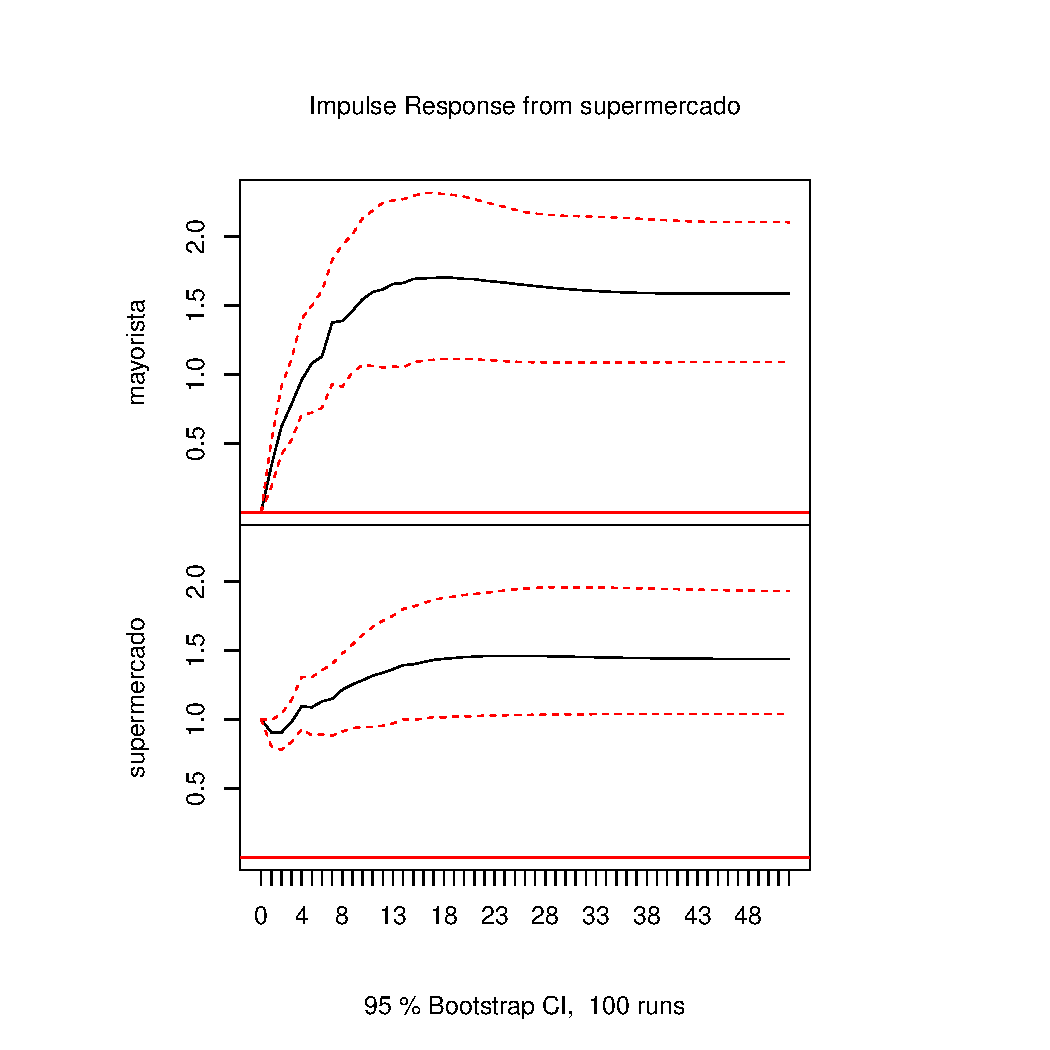
\includegraphics[width=4.5in,height=3.5in]{figure/graph5_7-2} 

}

\caption{Función acumulada de impulso respuesta\label{graph5.7}}\label{fig:graph5.72}
\end{figure}


\end{knitrout}


\section{Diagnósticos del modelo lineal}

\begin{knitrout}
\definecolor{shadecolor}{rgb}{0.969, 0.969, 0.969}\color{fgcolor}\begin{figure}[H]

{\centering 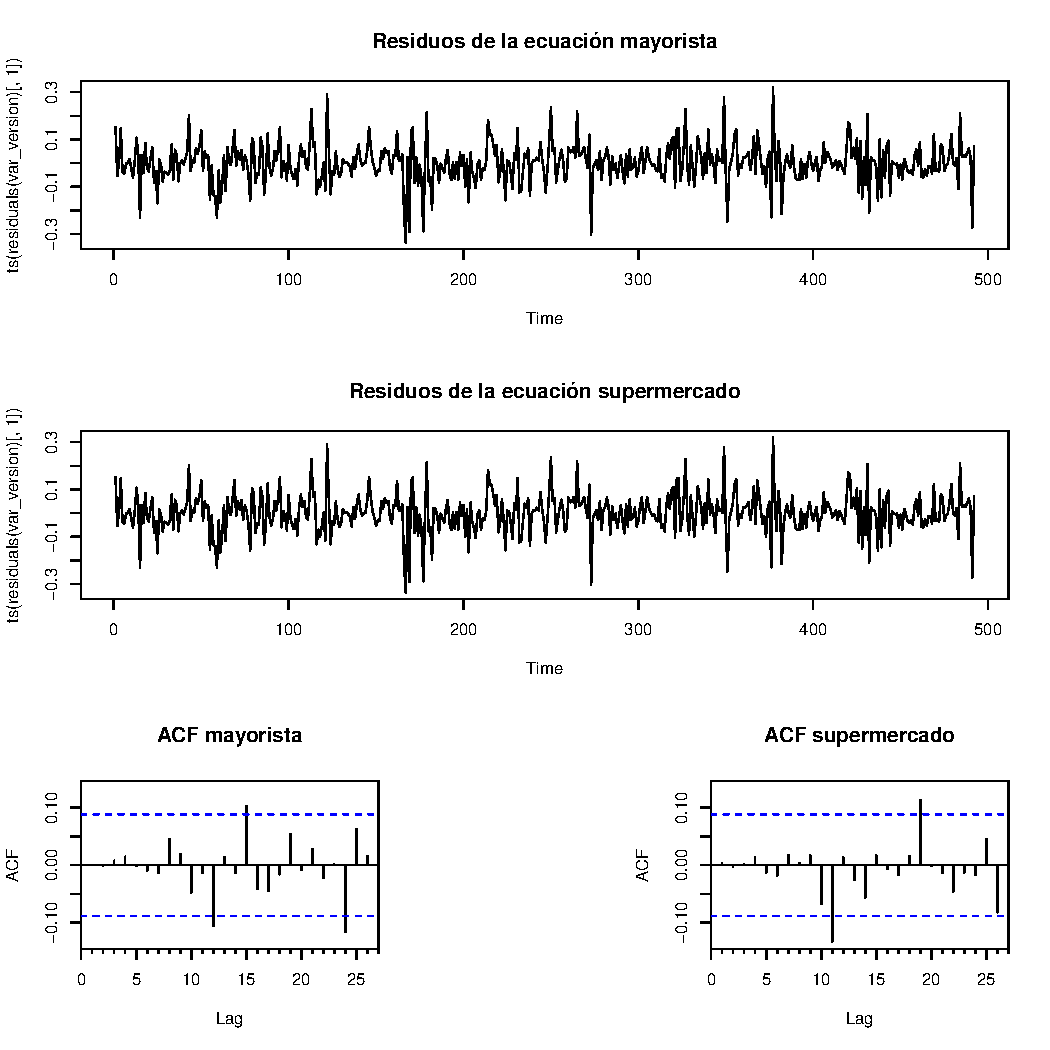
\includegraphics[width=4.5in,height=3.5in]{figure/graph5_8-1} 

}

\caption{Residuos del modelo\label{graph5.8}}\label{fig:graph5.8}
\end{figure}


\end{knitrout}




\begin{knitrout}
\definecolor{shadecolor}{rgb}{0.969, 0.969, 0.969}\color{fgcolor}\begin{figure}[H]

{\centering 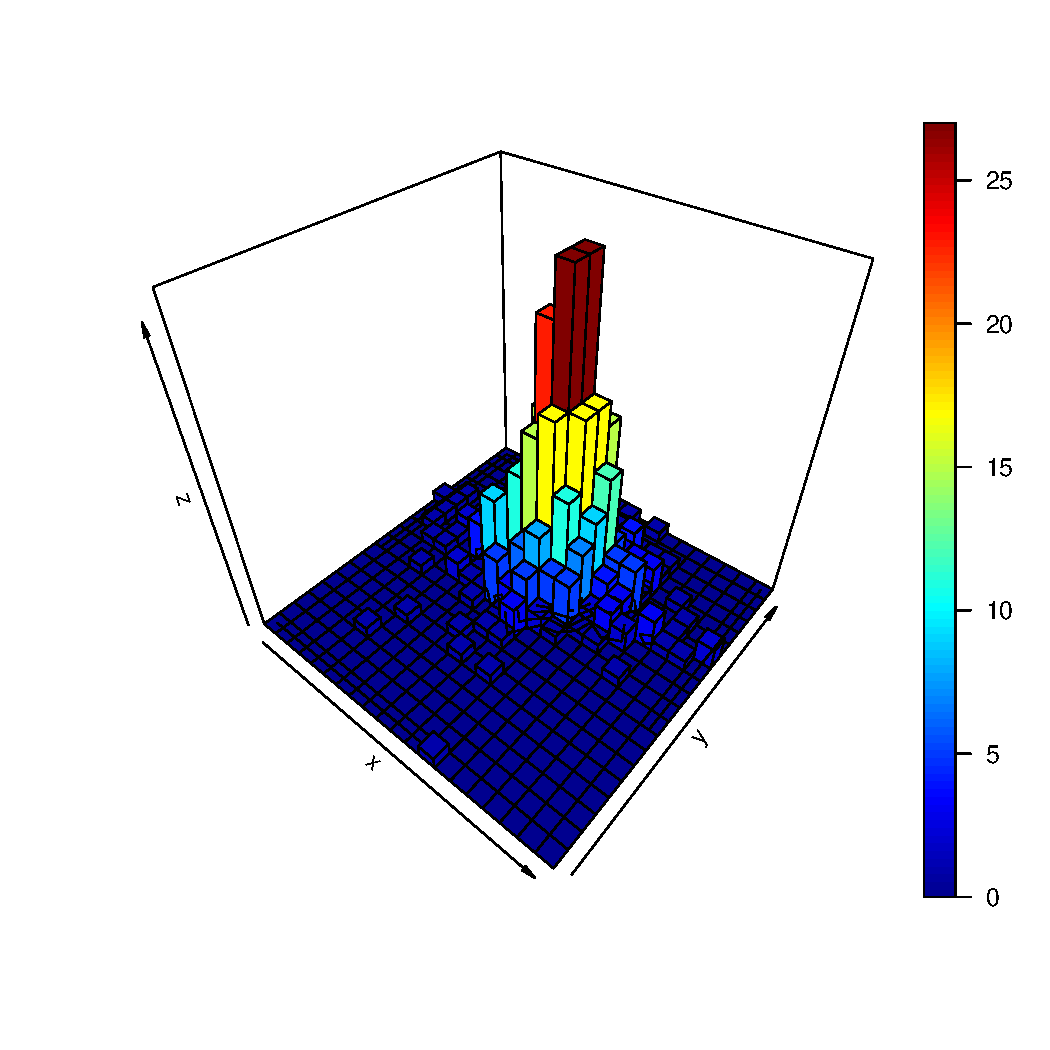
\includegraphics[width=3.5in,height=3.5in]{figure/fig-5_3_1-1} 

}

\caption[Histograma bivariado de los residuos del modelo]{Histograma bivariado de los residuos del modelo}\label{fig:fig-5.3.1}
\end{figure}


\end{knitrout}

\begin{knitrout}
\definecolor{shadecolor}{rgb}{0.969, 0.969, 0.969}\color{fgcolor}\begin{figure}[H]

{\centering 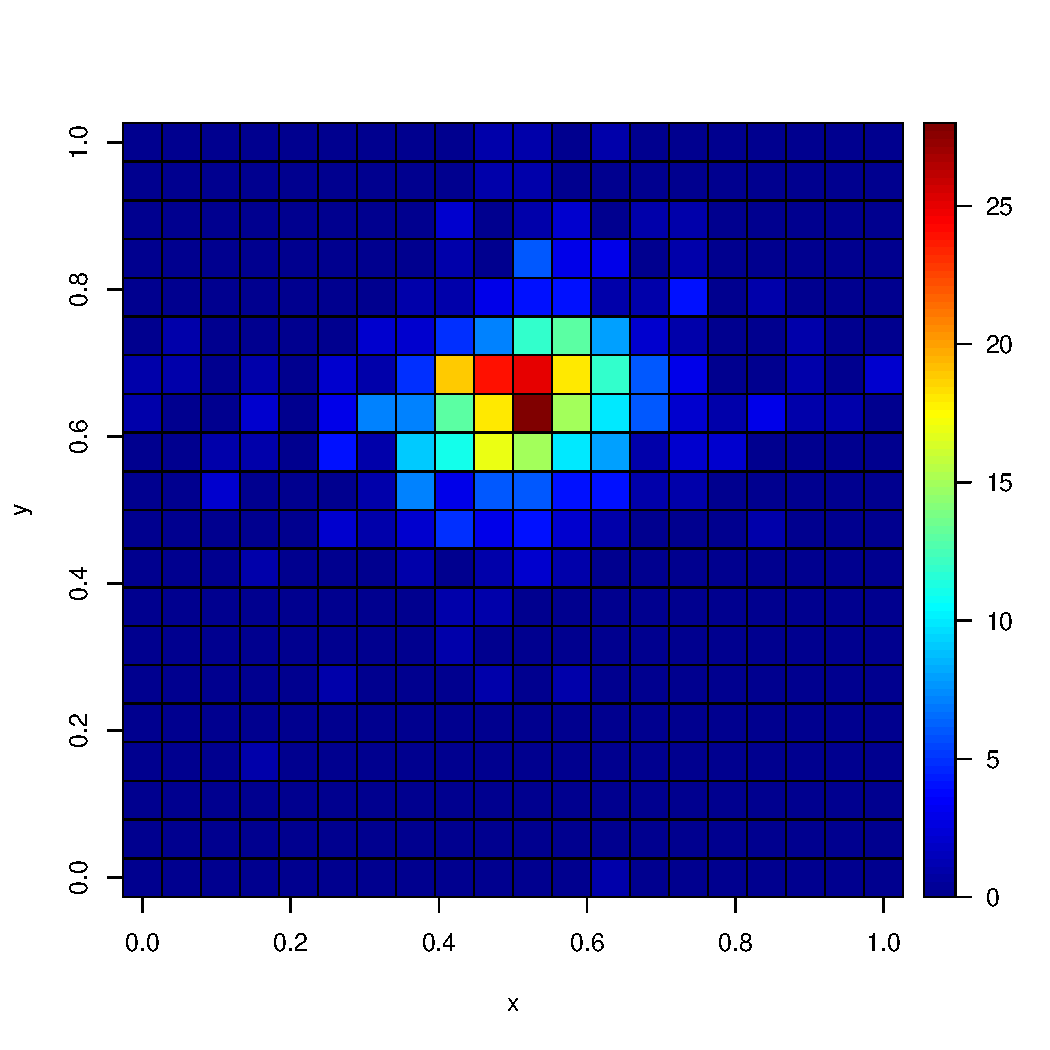
\includegraphics[width=3.5in,height=3.5in]{figure/fig-5_3_2-1} 

}

\caption[Mapa de calor de los residuos del modelo]{Mapa de calor de los residuos del modelo}\label{fig:fig-5.3.2}
\end{figure}


\end{knitrout}




\begin{table}[h]
\centering
\caption{Diagnósticos del modelo}
\begin{tabular}{@{}llll@{}}
\toprule \\ 
Contraste   & $E$ & df & $\mathbb{P}(\chi^{2}>E)$ \\
\midrule \\ 
Doornik \& Hansen & 246.913 & 4 & 2.11$\times 10^{-45}$ \\
Jarque-Bera (Multivariado) & 30.141 & 4 & $<$2.85$\times 10^{-7}$ \\
ARCH (Multivariado) & 144.4 & 81 & 1.89$\times 10^{-5}$ \\ 
\bottomrule 
\end{tabular}
\end{table}

\section{Determinación del rango de cointegración y estimación del modelo del modelo lineal de corrección del error}

Los contrastes y estimaciones de esta sección fueron realizadas a través del paquete \texttt{tsDyn} de Di Narzo, Aznarte \& Stigler(2009).


\begin{knitrout}
\definecolor{shadecolor}{rgb}{0.969, 0.969, 0.969}\color{fgcolor}\begin{kframe}
\begin{verbatim}
## 9588 (95.9%) points of the grid lead to regimes with percentage of observations < trim and were not computed
\end{verbatim}
\end{kframe}\begin{figure}[H]

{\centering 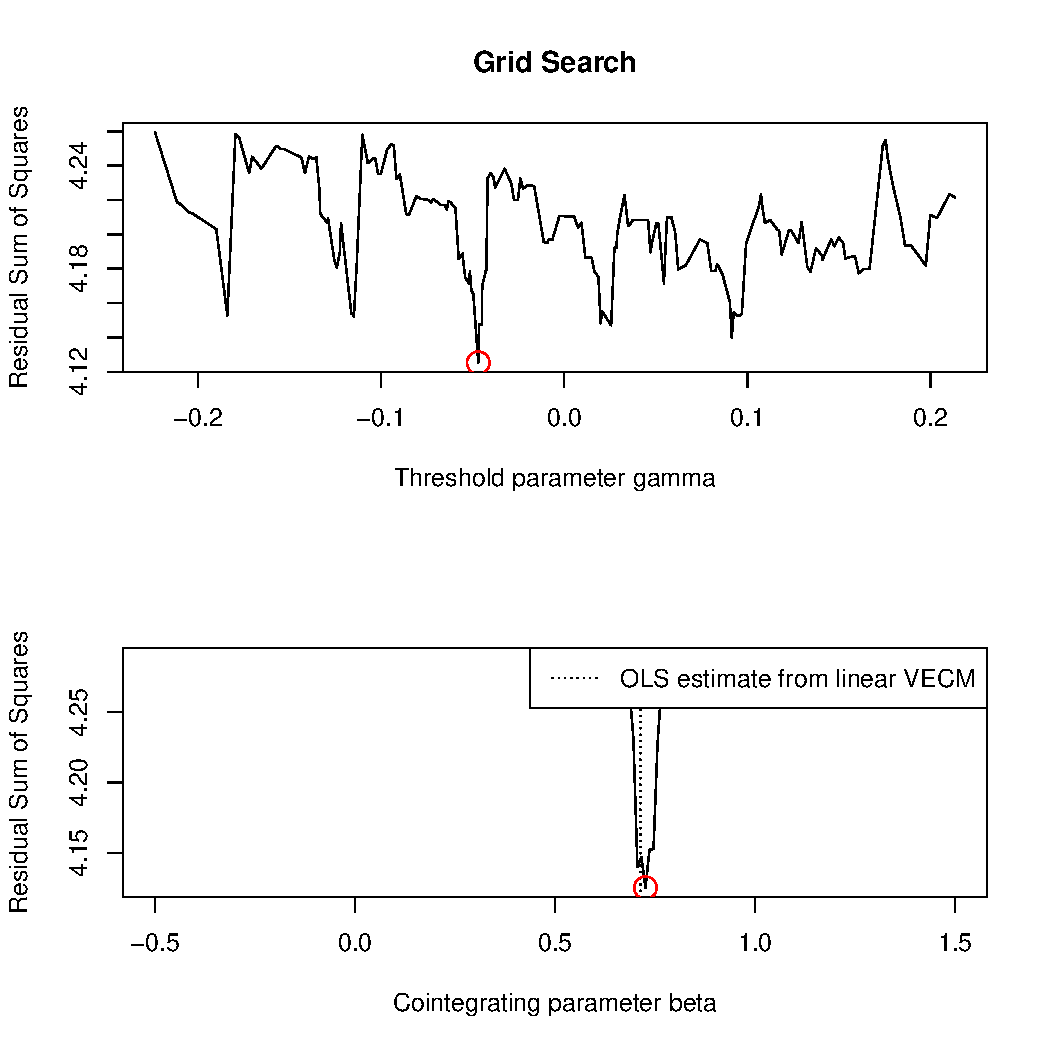
\includegraphics[width=4.5in,height=4.5in]{figure/fig-5_9-1} 

}

\caption[Modelo de corrección del error por umbrales]{Modelo de corrección del error por umbrales}\label{fig:fig-5.9}
\end{figure}


\end{knitrout}


\begin{knitrout}
\definecolor{shadecolor}{rgb}{0.969, 0.969, 0.969}\color{fgcolor}\begin{kframe}
\begin{verbatim}
## 1 (1%) points of the grid lead to regimes with percentage of observations < trim and were not computed
\end{verbatim}
\end{kframe}

{\centering 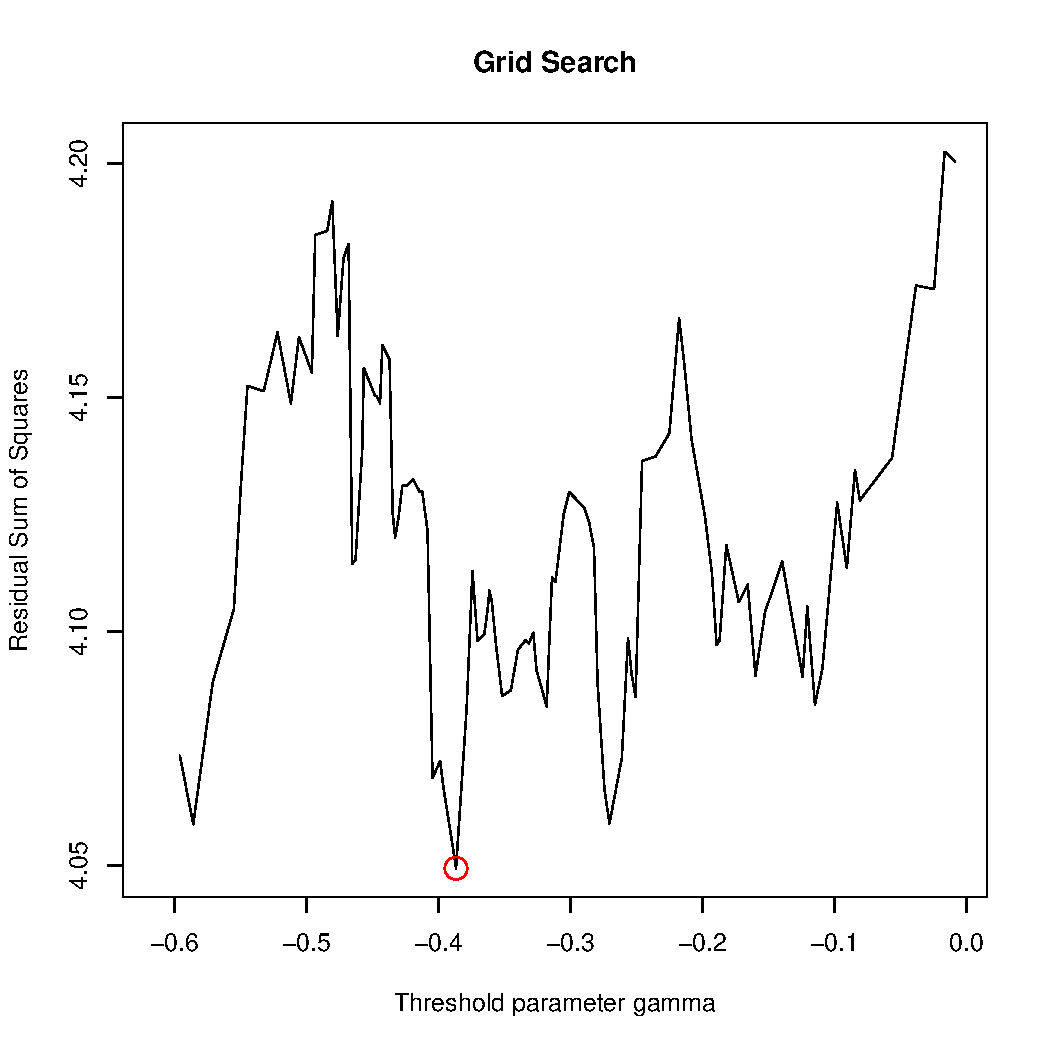
\includegraphics[width=4.5in,height=3.5in]{figure/Modelo_restringido-1} 

}



\end{knitrout}


\begin{knitrout}
\definecolor{shadecolor}{rgb}{0.969, 0.969, 0.969}\color{fgcolor}\begin{kframe}
\begin{verbatim}
## [1] 0.9982959
\end{verbatim}
\end{kframe}
\end{knitrout}


\begin{knitrout}
\definecolor{shadecolor}{rgb}{0.969, 0.969, 0.969}\color{fgcolor}

{\centering 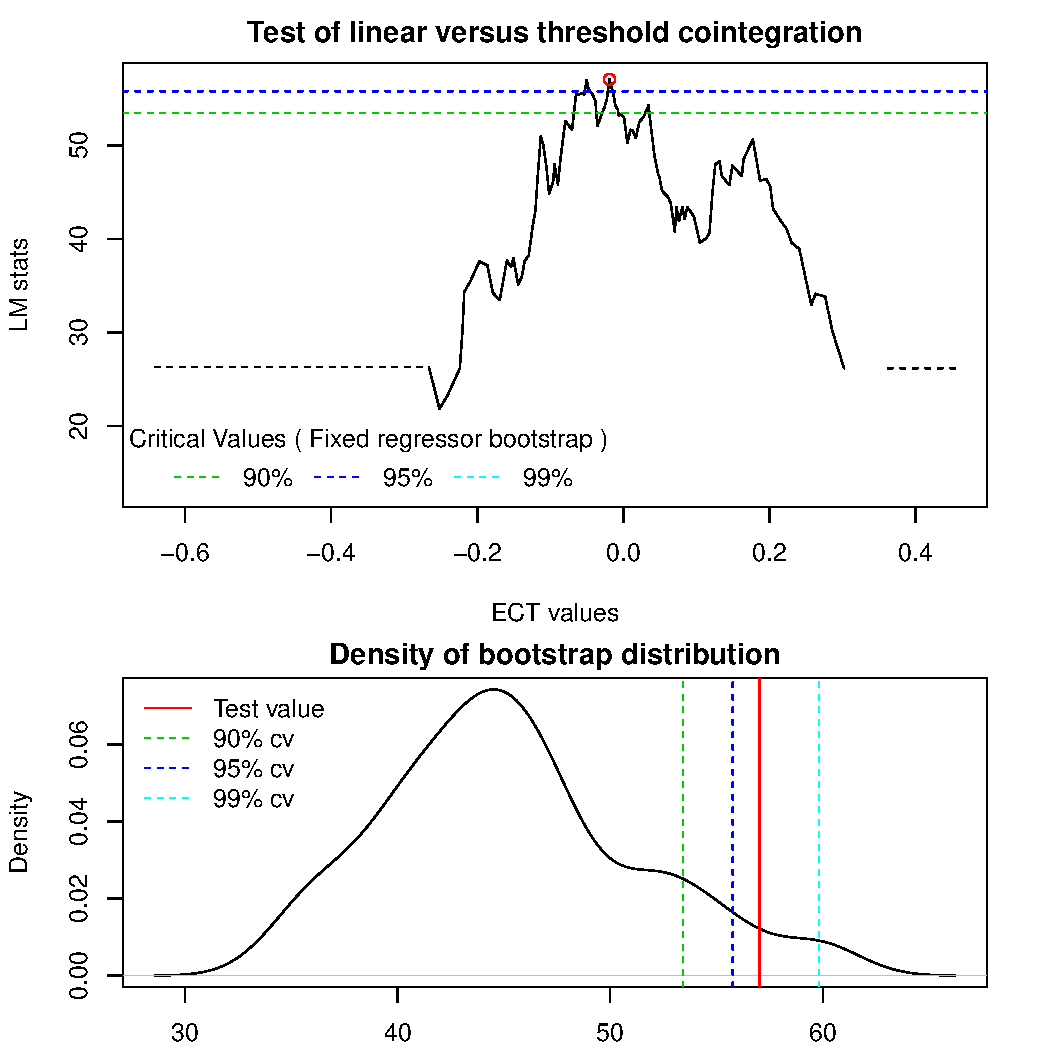
\includegraphics[width=4.5in,height=3.5in]{figure/unnamed-chunk-25-1} 

}



\end{knitrout}

\section{Diagnósticos del modelo no lineal}


\begin{knitrout}
\definecolor{shadecolor}{rgb}{0.969, 0.969, 0.969}\color{fgcolor}

{\centering 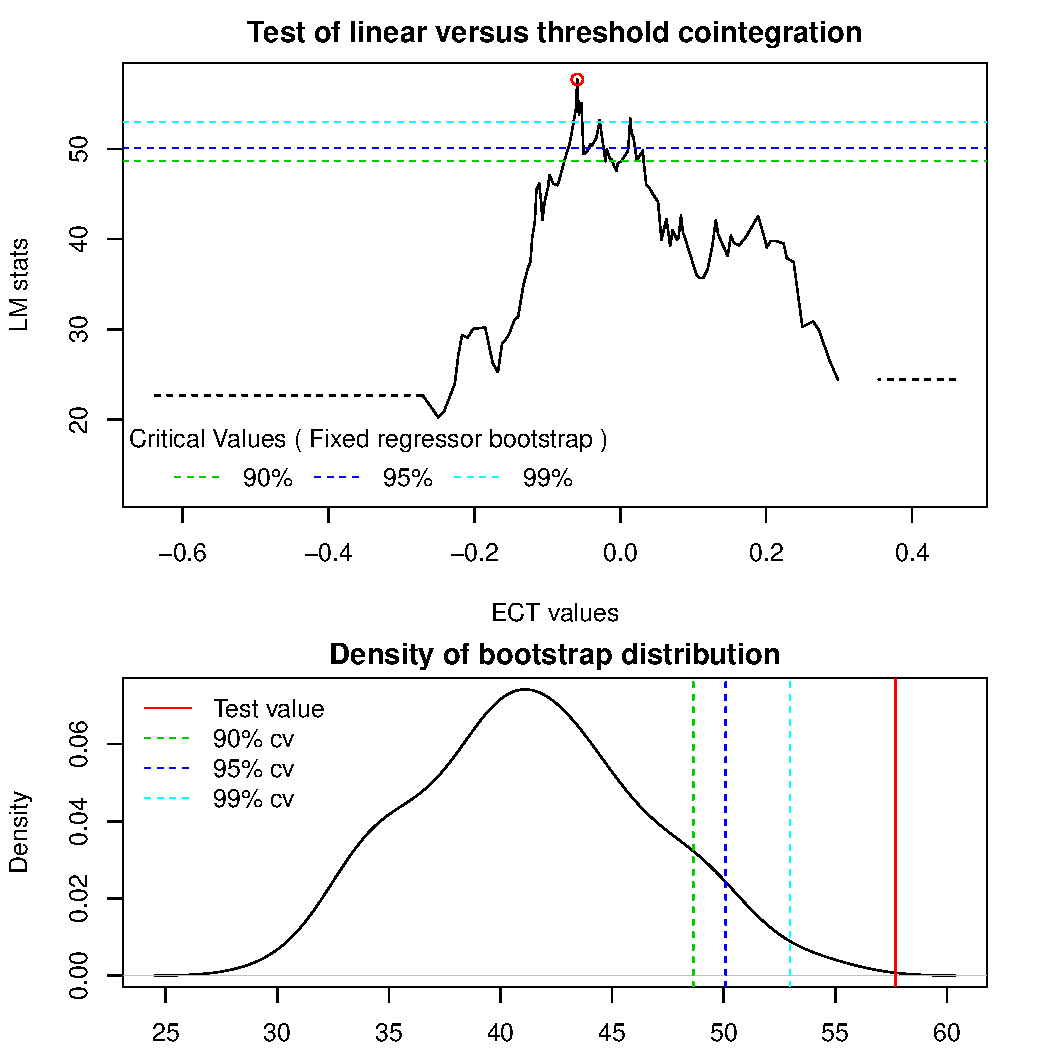
\includegraphics[width=4.5in,height=3.5in]{figure/unnamed-chunk-26-1} 

}



\end{knitrout}


\begin{knitrout}
\definecolor{shadecolor}{rgb}{0.969, 0.969, 0.969}\color{fgcolor}\begin{figure}[H]

{\centering 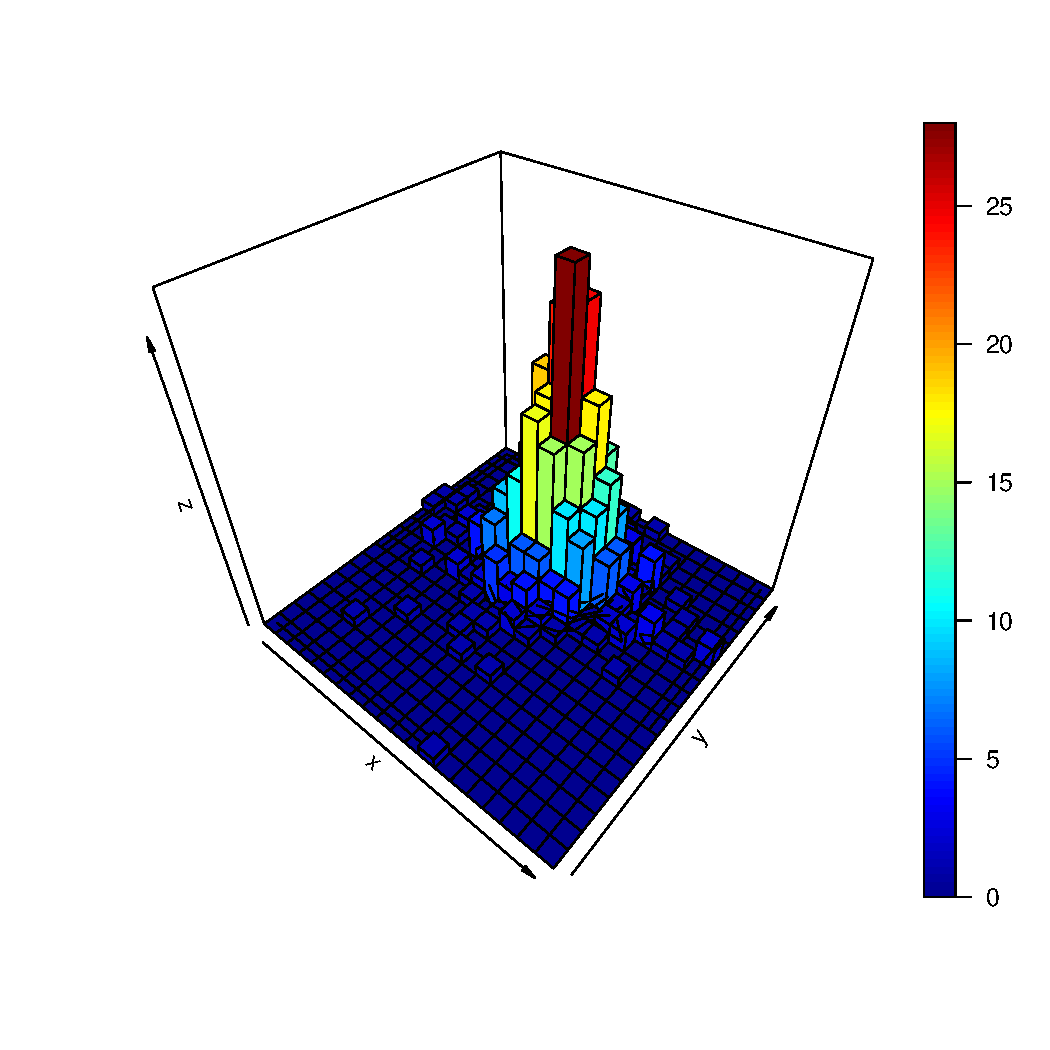
\includegraphics[width=3.5in,height=3.5in]{figure/fig-5_11-1} 

}

\caption[Histograma bivariado de los residuos del modelo]{Histograma bivariado de los residuos del modelo}\label{fig:fig-5.11}
\end{figure}


\end{knitrout}

\begin{knitrout}
\definecolor{shadecolor}{rgb}{0.969, 0.969, 0.969}\color{fgcolor}\begin{figure}[H]

{\centering 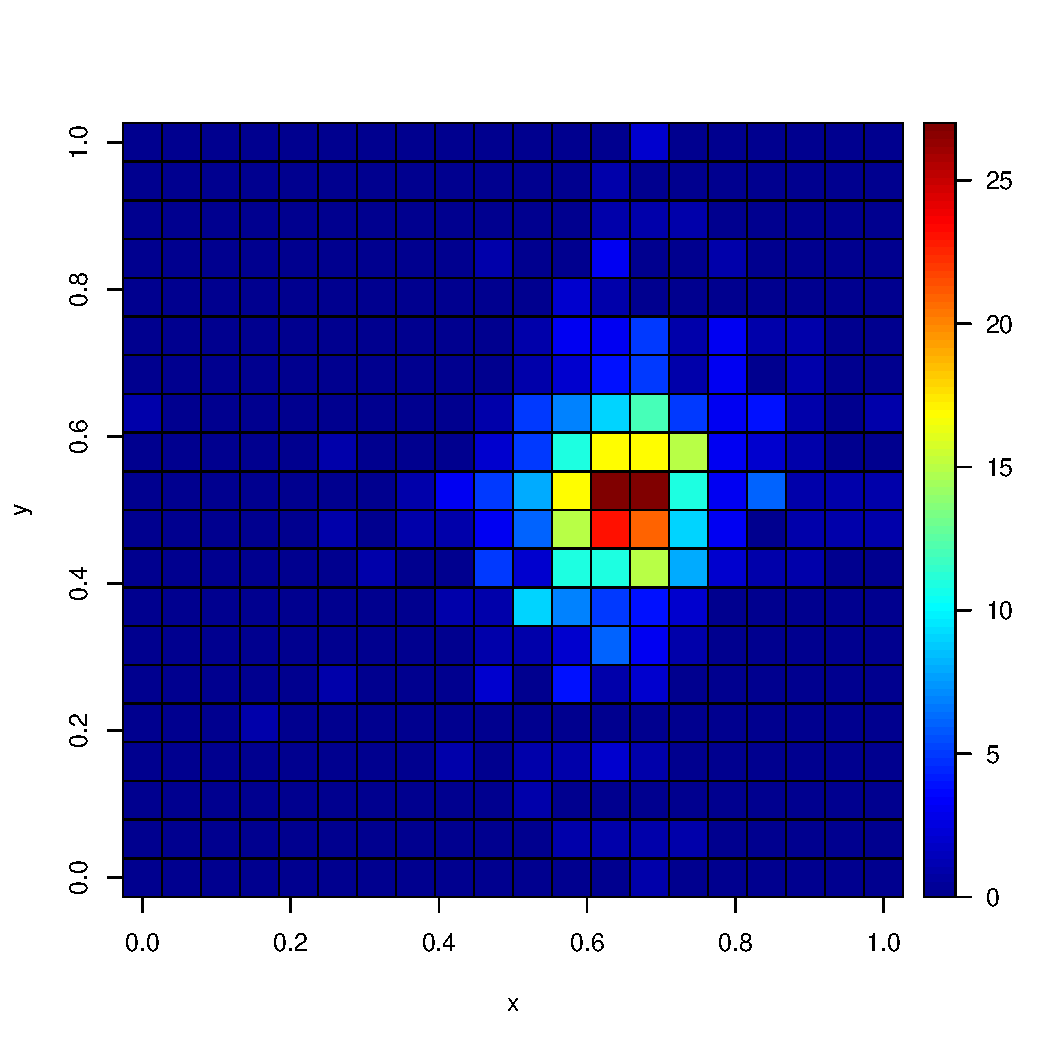
\includegraphics[width=3.5in,height=3.5in]{figure/fig-5_12-1} 

}

\caption[Mapa de calor de los residuos del modelo]{Mapa de calor de los residuos del modelo}\label{fig:fig-5.12}
\end{figure}


\end{knitrout}


\begin{knitrout}
\definecolor{shadecolor}{rgb}{0.969, 0.969, 0.969}\color{fgcolor}\begin{kframe}
\begin{verbatim}
## $multi
##          E df   P(Chi > E)
## 1 163.5603  4 2.519119e-34
## 
## $univ
##                      E df   P(Chi > E)
## mayorista     53.13165  2 2.901401e-12
## supermercado 110.42869  2 1.048853e-24
## $JB
## 
## 	JB-Test (multivariate)
## 
## data:  Residuals of VAR object mono_rest
## Chi-squared = 305.24, df = 4, p-value < 2.2e-16
## 
## 
## $Skewness
## 
## 	Skewness only (multivariate)
## 
## data:  Residuals of VAR object mono_rest
## Chi-squared = 12.421, df = 2, p-value = 0.002008
## 
## 
## $Kurtosis
## 
## 	Kurtosis only (multivariate)
## 
## data:  Residuals of VAR object mono_rest
## Chi-squared = 292.82, df = 2, p-value < 2.2e-16
## 
## 	ARCH (multivariate)
## 
## data:  Residuals of VAR object mono_rest
## Chi-squared = 121.29, df = 72, p-value = 0.000251
\end{verbatim}
\end{kframe}
\end{knitrout}


\chapter{Conclusiones}
\chapter{Bibliografía}

\hangindent=5em
\hangafter=-2

Ben-Kaabia, M., \& Gil Roig, J. M. (2008). Asimetrías en la transmisión de precios en el sector del tomate en España. Economía Agraria y Recursos Naturales, 8(1), 57-82.

Box, G. E., Jenkins, G. M., Reinsel, G. C., \& Ljung, G. M. (2015). Time series analysis: forecasting and control. John Wiley \& Sons.

Di Narzo, A. F., Aznarte, J. L., \& Stigler, M. (2009). tsDyn: Time series analysis based on dynamical systems theory. R package version 0.7.(URL: http://stat. ethz. ch/CRAN/web/packages/tsDyn/vignettes/tsDyn. pdf}.

Durbin, J., & Koopman, S. J. (2012). Time series analysis by state space methods (Vol. 38). OUP Oxford.

Hansen, B. E., \& Seo, B. (2002). Testing for two-regime threshold cointegration in vector error-correction models. Journal of econometrics, 110(2), 293-318.

Hyndman, R. J., \& Khandakar, Y. (2007). Automatic time series for forecasting: the forecast package for R (No. 6/07). Monash University, Department of Econometrics and Business Statistics.

Juselius, K. (2006). The cointegrated VAR model: methodology and applications. Oxford university press.

Kreiss, J. P., \& Lahiri, S. N. (2012). Bootstrap methods for time series. In Handbook of statistics (Vol. 30, pp. 3-26). Elsevier.

Lo, M. C., & Zivot, E. (2001). Threshold cointegration and nonlinear adjustment to the law of one price. Macroeconomic Dynamics, 5(4), 533-576.

Lütkepohl, H. (2005). New introduction to multiple time series analysis. Springer Science & Business Media.

Meyer, J., & Cramon‐Taubadel, S. (2004). Asymmetric price transmission: a survey. Journal of agricultural economics, 55(3), 581-611.

 Pfaff, B. (2008). VAR, SVAR and SVEC models: Implementation within R package vars. Journal of Statistical Software, 27(4), 1-32.

R Core Team (2017). R: A language and environment for statistical computing.
  R Foundation for Statistical Computing, Vienna, Austria. URL
  https://www.R-project.org/.

  
\chapter{Anexo}
\section{Algunos resultados útiles de cálculo matricial}

\subsection{Derivada de una forma cuadrática}
La traza de una matriz cuadrada $\mathbf{A}$ se define como la suma de los elementos de la diagonal $a_{ii}$ de $\mathbf{A}$: 

\begin{equation}
tr[\mathbf{A}]:= \sum_{i}a_{ii}
\end{equation}
Una propiedad útil de la traza es su invariabilidad antes permutaciones

\begin{teorema}
Sean $\mathbf{A,B,C}$ matrices cuadras de $n\times n$, se tiene que
\begin{equation}
tr[\mathbf{ABC}] = tr[\mathbf{CAB}] = tr[\mathbf{BCA}]
\end{equation}
\end{teorema}

\begin{teorema}
Sean $\mathbf{x} = \left[\begin{array}{c} x_{1} \\ \vdots \\ x_{n} \end{array}\right]$ y $\mathbf{A} =
\left[\begin{array}{ccc}
a_{11} & \hdots & a_{1n} \\ 
\vdots & \ddots & \vdots \\ 
a_{n1} & \hdots & a_{nn}
\end{array}\right]$. Entonces

\begin{equation}
\mathbf{x}^{T}\mathbf{Ax} = \sum_{j=1}^{n}\sum_{i=1}^{n}a_{ij}x_{i}x_{j}
\end{equation}
\end{teorema}

\begin{teorema}
Sean $\mathbf{x} = \left[\begin{array}{c} x_{1} \\ \vdots \\ x_{n} \end{array}\right]$ y $\mathbf{A} =
\left[\begin{array}{ccc}
a_{11} & \hdots & a_{1n} \\ 
\vdots & \ddots & \vdots \\ 
a_{n1} & \hdots & a_{nn}
\end{array}\right]$. Entonces

\begin{equation}
\frac{\partial}{\partial \mathbf{A}}\mathbf{x}^{T}\mathbf{Ax} = 
\frac{\partial}{\partial \mathbf{A}}tr\left[\mathbf{xx}^{T}\mathbf{A}\right] = \left[\mathbf{xx}^{T}\right]^{T} = \mathbf{xx}^{T}
\end{equation}

\end{teorema}
\subsection{Derivada de un determinante}

\begin{teo}{Formula de Jacobi}

Para cualquier matriz $A$

\end{teo}

\end{document}


